
    %% For double-blind review submission, w/o CCS and ACM Reference (max submission space)
\documentclass[sigplan,10pt,nonacm]{acmart}
% \documentclass[sigplan,10pt,review,nonacm]{acmart}

\settopmatter{printfolios=true,printccs=false,printacmref=false}

\usepackage[]{hyperref}
\usepackage{graphicx}
\usepackage{algorithm}
\usepackage{algpseudocode}
\usepackage{soul}
\usepackage{color}
\usepackage{enumitem}
\usepackage{algorithm}
\usepackage{algpseudocode}
\usepackage{multirow}
\usepackage{xcolor} % For color definitions
\usepackage{hyperref} % To handle citations inside highlights
\hypersetup{hidelinks} % Ensure links do not interfere
% \usepackage{ulem} % For underlining, which helps with compatibility

\soulregister{\cite}{7} % To allow citations inside \hl or \colorbox
\soulregister{\ref}{7}  % To allow references inside \hl or \colorbox
\soulregister{\pageref}{7} % To allow page references inside \hl

\algnewcommand{\LeftComment}[1]{\Statex \(\triangleright\) #1}

\algnewcommand\algorithmicforeach{\textbf{for each}}
\algdef{S}[FOR]{ForEach}[1]{\algorithmicforeach\ #1\ \algorithmicdo}

\acmConference[PL'18]{ACM SIGPLAN Conference on Programming Languages}{January 01--03, 2018}{New York, NY, USA}
\acmYear{2018}
\acmISBN{} % \acmISBN{978-x-xxxx-xxxx-x/YY/MM}
\acmDOI{} % \acmDOI{10.1145/nnnnnnn.nnnnnnn}
\startPage{1}
\setcopyright{none}
\bibliographystyle{ACM-Reference-Format}
\usepackage{booktabs}   %% For formal tables:
\usepackage{subcaption} %% For complex figures with 

\algblock{ParFor}{EndParFor}
% customizing the new block
\algnewcommand\algorithmicparfor{\textbf{parfor}}
\algnewcommand\algorithmicpardo{\textbf{do}}
\algnewcommand\algorithmicendparfor{\textbf{end\ parfor}}
\algrenewtext{ParFor}[1]{\algorithmicparfor\ #1\ \algorithmicpardo}
\algrenewtext{EndParFor}{\algorithmicendparfor}

\newcommand{\todo}[1]{\textcolor{blue}{(Zhijia: #1)}}

\begin{document}

% Title information
\title[]{Analysis of Stable Vertex Values: \\ Fast Query Evaluation Over An Evolving Graph} 

% \title[UVVs: Unchanged Vertex Values]{
% UVVs: Identifying Unchanged Vertex Values in \\ Evolving Graphs via Intersection-Union Analysis}

\author{Mahbod Afarin}
\authornote{Both authors contributed equally to this research.}
\email{mafar001@ucr.edu}
\affiliation{%
  \institution{CSE Department, UC Riverside}
  \country{USA}
}

\author{Chao Gao}
\authornotemark[1]
\email{cgao037@ucr.edu}
\affiliation{%
  \institution{CSE Department, UC Riverside}
  \country{USA}
}

\author{Xizhe Yin}
\email{xyin014@ucr.edu}
\affiliation{%
  \institution{CSE Department, UC Riverside}
  \country{USA}
}

\author{Zhijia Zhao}
\email{zhijia@cs.ucr.edu}
\affiliation{%
  \institution{CSE Department, UC Riverside}
  \country{USA}
}

\author{Nael Abu-Ghazaleh}
\email{nael@cs.ucr.edu}
\affiliation{%
  \institution{CSE Department, UC Riverside}
  \country{USA}
}

\author{Rajiv Gupta}
\email{rajivg@ucr.edu}
\affiliation{%
  \institution{CSE Department, UC Riverside}
  \country{USA}
}



\begin{abstract}
Evaluating a query over a large, irregular graph is inherently challenging. This challenge intensifies when solving a query over a sequence of snapshots of an evolving graph, where changes occur through the addition and deletion of edges. We carried out a study that shows that due to the gradually changing nature of evolving graphs, when a vertex-specific query (e.g., SSSP) is evaluated over a sequence of 25 to 100 snapshots, for 53.2\% to 99.8\% of vertices, the query results remain unchanged across all snapshots. Therefore, the \emph{Unchanged Vertex Values} (UVVs) can be computed once and then minimal analysis can be performed for each snapshot to obtain the results for the remaining vertices in that snapshot. We develop a novel \emph{intersection-union analysis} that very accurately computes lower and upper bounds of vertex values across all snapshots. When the lower and upper bounds for a vertex are found to be equal, we can safely conclude that the value found for the vertex remains the same across all snapshots. Therefore, the rest of our query evaluation is limited to computing values across snapshots for vertices whose bounds do not match.  We optimize this latter step evaluation by concurrently performing incremental computations on all snapshots over a significantly smaller subgraph. Our experiments with several benchmarks and graphs show that we need to carry out per snapshot incremental analysis for under 42\% vertices on a graph with under 32\% of edges. Our approach delivers speedups of 2.01-12.23$\times$ when compared to the state-of-the-art RisGraph implementation of the KickStarter-based incremental algorithm for 64 snapshots.

\end{abstract}

% \begin{CCSXML}
% <ccs2012>
% <concept>
% <concept_id>10011007.10011006.10011008</concept_id>
% <concept_desc>Software and its engineering~General programming languages</concept_desc>
% <concept_significance>500</concept_significance>
% </concept>
% <concept>
% <concept_id>10003456.10003457.10003521.10003525</concept_id>
% <concept_desc>Social and professional topics~History of programming languages</concept_desc>
% <concept_significance>300</concept_significance>
% </concept>
% </ccs2012>
% \end{CCSXML}

% \ccsdesc[500]{Software and its engineering~General programming languages}
% \ccsdesc[300]{Social and professional topics~History of programming languages}
%% End of generated code


%% Keywords
%% comma separated list
% \keywords{evolving graphs, graph intersection, graph union, monotonic graph algorithms}  %% \keywords are mandatory in final camera-ready submission

\maketitle 
% \pagestyle{plain} % should come right after \maketitle

\section{Introduction}

Large language models (LLMs) have achieved remarkable success in automated math problem solving, particularly through code-generation capabilities integrated with proof assistants~\citep{lean,isabelle,POT,autoformalization,MATH}. Although LLMs excel at generating solution steps and correct answers in algebra and calculus~\citep{math_solving}, their unimodal nature limits performance in plane geometry, where solution depends on both diagram and text~\citep{math_solving}. 

Specialized vision-language models (VLMs) have accordingly been developed for plane geometry problem solving (PGPS)~\citep{geoqa,unigeo,intergps,pgps,GOLD,LANS,geox}. Yet, it remains unclear whether these models genuinely leverage diagrams or rely almost exclusively on textual features. This ambiguity arises because existing PGPS datasets typically embed sufficient geometric details within problem statements, potentially making the vision encoder unnecessary~\citep{GOLD}. \cref{fig:pgps_examples} illustrates example questions from GeoQA and PGPS9K, where solutions can be derived without referencing the diagrams.

\begin{figure}
    \centering
    \begin{subfigure}[t]{.49\linewidth}
        \centering
        \includegraphics[width=\linewidth]{latex/figures/images/geoqa_example.pdf}
        \caption{GeoQA}
        \label{fig:geoqa_example}
    \end{subfigure}
    \begin{subfigure}[t]{.48\linewidth}
        \centering
        \includegraphics[width=\linewidth]{latex/figures/images/pgps_example.pdf}
        \caption{PGPS9K}
        \label{fig:pgps9k_example}
    \end{subfigure}
    \caption{
    Examples of diagram-caption pairs and their solution steps written in formal languages from GeoQA and PGPS9k datasets. In the problem description, the visual geometric premises and numerical variables are highlighted in green and red, respectively. A significant difference in the style of the diagram and formal language can be observable. %, along with the differences in formal languages supported by the corresponding datasets.
    \label{fig:pgps_examples}
    }
\end{figure}



We propose a new benchmark created via a synthetic data engine, which systematically evaluates the ability of VLM vision encoders to recognize geometric premises. Our empirical findings reveal that previously suggested self-supervised learning (SSL) approaches, e.g., vector quantized variataional auto-encoder (VQ-VAE)~\citep{unimath} and masked auto-encoder (MAE)~\citep{scagps,geox}, and widely adopted encoders, e.g., OpenCLIP~\citep{clip} and DinoV2~\citep{dinov2}, struggle to detect geometric features such as perpendicularity and degrees. 

To this end, we propose \geoclip{}, a model pre-trained on a large corpus of synthetic diagram–caption pairs. By varying diagram styles (e.g., color, font size, resolution, line width), \geoclip{} learns robust geometric representations and outperforms prior SSL-based methods on our benchmark. Building on \geoclip{}, we introduce a few-shot domain adaptation technique that efficiently transfers the recognition ability to real-world diagrams. We further combine this domain-adapted GeoCLIP with an LLM, forming a domain-agnostic VLM for solving PGPS tasks in MathVerse~\citep{mathverse}. 
%To accommodate diverse diagram styles and solution formats, we unify the solution program languages across multiple PGPS datasets, ensuring comprehensive evaluation. 

In our experiments on MathVerse~\citep{mathverse}, which encompasses diverse plane geometry tasks and diagram styles, our VLM with a domain-adapted \geoclip{} consistently outperforms both task-specific PGPS models and generalist VLMs. 
% In particular, it achieves higher accuracy on tasks requiring geometric-feature recognition, even when critical numerical measurements are moved from text to diagrams. 
Ablation studies confirm the effectiveness of our domain adaptation strategy, showing improvements in optical character recognition (OCR)-based tasks and robust diagram embeddings across different styles. 
% By unifying the solution program languages of existing datasets and incorporating OCR capability, we enable a single VLM, named \geovlm{}, to handle a broad class of plane geometry problems.

% Contributions
We summarize the contributions as follows:
We propose a novel benchmark for systematically assessing how well vision encoders recognize geometric premises in plane geometry diagrams~(\cref{sec:visual_feature}); We introduce \geoclip{}, a vision encoder capable of accurately detecting visual geometric premises~(\cref{sec:geoclip}), and a few-shot domain adaptation technique that efficiently transfers this capability across different diagram styles (\cref{sec:domain_adaptation});
We show that our VLM, incorporating domain-adapted GeoCLIP, surpasses existing specialized PGPS VLMs and generalist VLMs on the MathVerse benchmark~(\cref{sec:experiments}) and effectively interprets diverse diagram styles~(\cref{sec:abl}).

\iffalse
\begin{itemize}
    \item We propose a novel benchmark for systematically assessing how well vision encoders recognize geometric premises, e.g., perpendicularity and angle measures, in plane geometry diagrams.
	\item We introduce \geoclip{}, a vision encoder capable of accurately detecting visual geometric premises, and a few-shot domain adaptation technique that efficiently transfers this capability across different diagram styles.
	\item We show that our final VLM, incorporating GeoCLIP-DA, effectively interprets diverse diagram styles and achieves state-of-the-art performance on the MathVerse benchmark, surpassing existing specialized PGPS models and generalist VLM models.
\end{itemize}
\fi

\iffalse

Large language models (LLMs) have made significant strides in automated math word problem solving. In particular, their code-generation capabilities combined with proof assistants~\citep{lean,isabelle} help minimize computational errors~\citep{POT}, improve solution precision~\citep{autoformalization}, and offer rigorous feedback and evaluation~\citep{MATH}. Although LLMs excel in generating solution steps and correct answers for algebra and calculus~\citep{math_solving}, their uni-modal nature limits performance in domains like plane geometry, where both diagrams and text are vital.

Plane geometry problem solving (PGPS) tasks typically include diagrams and textual descriptions, requiring solvers to interpret premises from both sources. To facilitate automated solutions for these problems, several studies have introduced formal languages tailored for plane geometry to represent solution steps as a program with training datasets composed of diagrams, textual descriptions, and solution programs~\citep{geoqa,unigeo,intergps,pgps}. Building on these datasets, a number of PGPS specialized vision-language models (VLMs) have been developed so far~\citep{GOLD, LANS, geox}.

Most existing VLMs, however, fail to use diagrams when solving geometry problems. Well-known PGPS datasets such as GeoQA~\citep{geoqa}, UniGeo~\citep{unigeo}, and PGPS9K~\citep{pgps}, can be solved without accessing diagrams, as their problem descriptions often contain all geometric information. \cref{fig:pgps_examples} shows an example from GeoQA and PGPS9K datasets, where one can deduce the solution steps without knowing the diagrams. 
As a result, models trained on these datasets rely almost exclusively on textual information, leaving the vision encoder under-utilized~\citep{GOLD}. 
Consequently, the VLMs trained on these datasets cannot solve the plane geometry problem when necessary geometric properties or relations are excluded from the problem statement.

Some studies seek to enhance the recognition of geometric premises from a diagram by directly predicting the premises from the diagram~\citep{GOLD, intergps} or as an auxiliary task for vision encoders~\citep{geoqa,geoqa-plus}. However, these approaches remain highly domain-specific because the labels for training are difficult to obtain, thus limiting generalization across different domains. While self-supervised learning (SSL) methods that depend exclusively on geometric diagrams, e.g., vector quantized variational auto-encoder (VQ-VAE)~\citep{unimath} and masked auto-encoder (MAE)~\citep{scagps,geox}, have also been explored, the effectiveness of the SSL approaches on recognizing geometric features has not been thoroughly investigated.

We introduce a benchmark constructed with a synthetic data engine to evaluate the effectiveness of SSL approaches in recognizing geometric premises from diagrams. Our empirical results with the proposed benchmark show that the vision encoders trained with SSL methods fail to capture visual \geofeat{}s such as perpendicularity between two lines and angle measure.
Furthermore, we find that the pre-trained vision encoders often used in general-purpose VLMs, e.g., OpenCLIP~\citep{clip} and DinoV2~\citep{dinov2}, fail to recognize geometric premises from diagrams.

To improve the vision encoder for PGPS, we propose \geoclip{}, a model trained with a massive amount of diagram-caption pairs.
Since the amount of diagram-caption pairs in existing benchmarks is often limited, we develop a plane diagram generator that can randomly sample plane geometry problems with the help of existing proof assistant~\citep{alphageometry}.
To make \geoclip{} robust against different styles, we vary the visual properties of diagrams, such as color, font size, resolution, and line width.
We show that \geoclip{} performs better than the other SSL approaches and commonly used vision encoders on the newly proposed benchmark.

Another major challenge in PGPS is developing a domain-agnostic VLM capable of handling multiple PGPS benchmarks. As shown in \cref{fig:pgps_examples}, the main difficulties arise from variations in diagram styles. 
To address the issue, we propose a few-shot domain adaptation technique for \geoclip{} which transfers its visual \geofeat{} perception from the synthetic diagrams to the real-world diagrams efficiently. 

We study the efficacy of the domain adapted \geoclip{} on PGPS when equipped with the language model. To be specific, we compare the VLM with the previous PGPS models on MathVerse~\citep{mathverse}, which is designed to evaluate both the PGPS and visual \geofeat{} perception performance on various domains.
While previous PGPS models are inapplicable to certain types of MathVerse problems, we modify the prediction target and unify the solution program languages of the existing PGPS training data to make our VLM applicable to all types of MathVerse problems.
Results on MathVerse demonstrate that our VLM more effectively integrates diagrammatic information and remains robust under conditions of various diagram styles.

\begin{itemize}
    \item We propose a benchmark to measure the visual \geofeat{} recognition performance of different vision encoders.
    % \item \sh{We introduce geometric CLIP (\geoclip{} and train the VLM equipped with \geoclip{} to predict both solution steps and the numerical measurements of the problem.}
    \item We introduce \geoclip{}, a vision encoder which can accurately recognize visual \geofeat{}s and a few-shot domain adaptation technique which can transfer such ability to different domains efficiently. 
    % \item \sh{We develop our final PGPS model, \geovlm{}, by adapting \geoclip{} to different domains and training with unified languages of solution program data.}
    % We develop a domain-agnostic VLM, namely \geovlm{}, by applying a simple yet effective domain adaptation method to \geoclip{} and training on the refined training data.
    \item We demonstrate our VLM equipped with GeoCLIP-DA effectively interprets diverse diagram styles, achieving superior performance on MathVerse compared to the existing PGPS models.
\end{itemize}

\fi 

\section{Background}\label{sec:backgrnd}

\subsection{Cold Start Latency and Mitigation Techniques}

Traditional FaaS platforms mitigate cold starts through snapshotting, lightweight virtualization, and warm-state management. Snapshot-based methods like \textbf{REAP} and \textbf{Catalyzer} reduce initialization time by preloading or restoring container states but require significant memory and I/O resources, limiting scalability~\cite{dong_catalyzer_2020, ustiugov_benchmarking_2021}. Lightweight virtualization solutions, such as \textbf{Firecracker} microVMs, achieve fast startup times with strong isolation but depend on robust infrastructure, making them less adaptable to fluctuating workloads~\cite{agache_firecracker_2020}. Warm-state management techniques like \textbf{Faa\$T}~\cite{romero_faa_2021} and \textbf{Kraken}~\cite{vivek_kraken_2021} keep frequently invoked containers ready, balancing readiness and cost efficiency under predictable workloads but incurring overhead when demand is erratic~\cite{romero_faa_2021, vivek_kraken_2021}. While these methods perform well in resource-rich cloud environments, their resource intensity challenges applicability in edge settings.

\subsubsection{Edge FaaS Perspective}

In edge environments, cold start mitigation emphasizes lightweight designs, resource sharing, and hybrid task distribution. Lightweight execution environments like unikernels~\cite{edward_sock_2018} and \textbf{Firecracker}~\cite{agache_firecracker_2020}, as used by \textbf{TinyFaaS}~\cite{pfandzelter_tinyfaas_2020}, minimize resource usage and initialization delays but require careful orchestration to avoid resource contention. Function co-location, demonstrated by \textbf{Photons}~\cite{v_dukic_photons_2020}, reduces redundant initializations by sharing runtime resources among related functions, though this complicates isolation in multi-tenant setups~\cite{v_dukic_photons_2020}. Hybrid offloading frameworks like \textbf{GeoFaaS}~\cite{malekabbasi_geofaas_2024} balance edge-cloud workloads by offloading latency-tolerant tasks to the cloud and reserving edge resources for real-time operations, requiring reliable connectivity and efficient task management. These edge-specific strategies address cold starts effectively but introduce challenges in scalability and orchestration.

\subsection{Predictive Scaling and Caching Techniques}

Efficient resource allocation is vital for maintaining low latency and high availability in serverless platforms. Predictive scaling and caching techniques dynamically provision resources and reduce cold start latency by leveraging workload prediction and state retention.
Traditional FaaS platforms use predictive scaling and caching to optimize resources, employing techniques (OFC, FaasCache) to reduce cold starts. However, these methods rely on centralized orchestration and workload predictability, limiting their effectiveness in dynamic, resource-constrained edge environments.



\subsubsection{Edge FaaS Perspective}

Edge FaaS platforms adapt predictive scaling and caching techniques to constrain resources and heterogeneous environments. \textbf{EDGE-Cache}~\cite{kim_delay-aware_2022} uses traffic profiling to selectively retain high-priority functions, reducing memory overhead while maintaining readiness for frequent requests. Hybrid frameworks like \textbf{GeoFaaS}~\cite{malekabbasi_geofaas_2024} implement distributed caching to balance resources between edge and cloud nodes, enabling low-latency processing for critical tasks while offloading less critical workloads. Machine learning methods, such as clustering-based workload predictors~\cite{gao_machine_2020} and GRU-based models~\cite{guo_applying_2018}, enhance resource provisioning in edge systems by efficiently forecasting workload spikes. These innovations effectively address cold start challenges in edge environments, though their dependency on accurate predictions and robust orchestration poses scalability challenges.

\subsection{Decentralized Orchestration, Function Placement, and Scheduling}

Efficient orchestration in serverless platforms involves workload distribution, resource optimization, and performance assurance. While traditional FaaS platforms rely on centralized control, edge environments require decentralized and adaptive strategies to address unique challenges such as resource constraints and heterogeneous hardware.



\subsubsection{Edge FaaS Perspective}

Edge FaaS platforms adopt decentralized and adaptive orchestration frameworks to meet the demands of resource-constrained environments. Systems like \textbf{Wukong} distribute scheduling across edge nodes, enhancing data locality and scalability while reducing network latency. Lightweight frameworks such as \textbf{OpenWhisk Lite}~\cite{kravchenko_kpavelopenwhisk-light_2024} optimize resource allocation by decentralizing scheduling policies, minimizing cold starts and latency in edge setups~\cite{benjamin_wukong_2020}. Hybrid solutions like \textbf{OpenFaaS}~\cite{noauthor_openfaasfaas_2024} and \textbf{EdgeMatrix}~\cite{shen_edgematrix_2023} combine edge-cloud orchestration to balance resource utilization, retaining latency-sensitive functions at the edge while offloading non-critical workloads to the cloud. While these approaches improve flexibility, they face challenges in maintaining coordination and ensuring consistent performance across distributed nodes.



%PlanGREEN

%GEN-Plan

%G- generate
%R-refine
%E- edit

%% GREEN-plan

%% PURPLE
\begin{figure*}
    \centering
    \Description{PLAID's system architecture diagram. Top part shows the database (a), and bottom part shows the interface (b). The system starts from bottom right as an instructor is interested in a programming domain, then the pipeline described in the text produces reference materials at different levels of granularity, and these are presented in the interface.}
    \includegraphics[width=\textwidth]{img/system-architecture-subgoals.png}
    \caption{PLAID's reference content is generated through an LLM pipeline
    %inspired by the practices of instructors who have successfully identified programming plans. 
    that produces output on three levels.
    First, a wide variety of use cases are generated to create example programs that focus on code's applications. Next, using LLM's explanatory comments that represent subgoals within the code, the examples are segmented into meaningful code snippets. The LLM is queried to generate other plan components for each code snippet. Finally, the code snippets are clustered to identify the most common patterns, representing plan candidates. The full programs are presented in `Programs' views of PLAID interface, whereas snippets are presented in clusters in the `Plan Creation' view.}
    \label{fig:system-pipeline}
\end{figure*}
\section{PLAID: A System for Supporting Plan Identification}
\label{sec:system-design}

Following the design goals devised from the design workshop, we refined our early prototype into PLAID: a
%LLM-powered
tool to assist instructors in their plan identification process.
PLAID synthesizes the capabilities of LLMs in code generation with interactions enabling plan identification practices observed in our studies with instructors.
As we noted in the findings of our design workshop, the LLM-generated candidate plans are not ready to be used as is in instruction, but instructors can readily adapt and correct them (\cref{sec:workshop-findings-condition2}).
PLAID enables collaboration between instructors and LLMs, enhancing the plan identification process by automating its time-intensive information-gathering tasks and facilitating instructors' ability to refine LLM-generated candidate plans based on their knowledge about pedagogy and the programming domain. 



\subsection{Practical Illustration}

To understand how instructors use can PLAID to more easily adopt plan-based pedagogies, we follow Jane, a computer science instructor using PLAID to design programming plans for her course (summarized in \cref{fig:jane-workflow}).

Jane is teaching a programming course for psychology majors and wants to introduce her students to data analysis using Pandas. As her students have limited prior programming experience and use programming for specific goals, she organizes her lecture material around programming plans to emphasize purpose over syntax. 
% that explain practical concepts to students and help them focus on the purpose behind the code they write.
% However, she realizes that all introductory computer science courses offered at her institution only teach basic programming constructs like data structures. After exploring Google Scholar for effective instructional methods to teach application-focused programming to non-computer science majors, she learned about plan-based pedagogies that help them focus on the purpose behind the code they write. In her literature review, she finds out about PLAID, a tool that can help her design domain-specific plans. She reviews the domains supported by the tool (Pandas, Pytorch, Beautifulsoup, and Django) and decides to use Pandas, a popular and powerful data analysis and manipulation library, to create her curriculum. 

She logs in to the PLAID web interface, % and takes time to explore the system's features. 
and asks PLAID to suggest a plan (\cref{fig:jane-workflow}, 1). The first plan recommended to her 
% she sees is a plan to help students learn about
is about reading CSV files. 
She thinks the topic is important and the solution code aligns with her experience; % the solution is promising and represents an important concept that students need to know about.
% She is satisfied with the given solution 
but she finds the generated name and goal to be too generic. She edits (\cref{fig:jane-workflow}, 2) these fields to provide more context that she feels is right for her students.
% She refines those fields and then 
To make this plan more abstract and appropriate for more use cases, %explain how this plan can be used for reading data from different file formats,
she marks the file path as a changeable area (\cref{fig:jane-workflow}, 3), generalizing the plan for reading data from different file formats.

Inspired by the first plan, she decides to create a plan for saving data to disk. She wants to teach the most conventional way of saving data, so she switches to the use case tab (\cref{fig:jane-workflow}, 4) and explores example programs that save data to get a sense of common practices.  %interact with the list of complete programs.
She finds a complete example where a DataFrame is created and and saved to a file. %performs cleaning tasks like deleting NaN values, and exports it.
% She realizes that something she hadn't thought of before: saving new data is almost always necessary after performing data manipulation operations!
She selects the part of the code that exports data to a file and creates a plan from that selection (\cref{fig:jane-workflow}, 5).


For the next plan, she reflects on her own experience with Pandas. She recalls that merging DataFrames was a key concept, but cannot remember the full syntax. 
% Jane reflects on her experience working with Pandas and recalls that merging DataFrames is a key operation when working with big data.
She switches to the full programs tab (\cref{fig:jane-workflow}, 6) that includes complete code examples and searches (\cref{fig:jane-workflow}, 7) for ``\texttt{.merge}'' to find different instances of merging operations. % and tries to use the search bar to find a relevant program that contains ``.merge''. 
After finding a comprehensive example, she selects the relevant section of the code and creates a plan from it.
% She again selects a part of the example, creates plan from the selection, and refines it. She engages with the system iteratively and designs twenty plans for her lecture. 

After designing a set of plans that capture the important topics, she organizes them into groups (\cref{fig:jane-workflow}, 8) 
% also grouped similar plans together
to emphasize sets of plans with similar goals but different implementations. For instance, she takes her plans about \texttt{.merge} and \texttt{.concat} and groups them together to form a category of plans that students can reference when they want to {combine data from different sources}.

% combining data using ``merge'' or ``concat''.

% the the she used plans isn't very good right now
% She exports these plans and starts preparing her lecture slides, using the plans as a way of presenting key concepts to students with minimal programming experience.
She exports these plans to support her students with minimal programming experience by preparing lecture slides that organize the sections around plan goals, using plan solutions as worked examples in class, and providing students with cheat sheets that include relevant plans for their laboratory sessions.
% using the plan goals as titles for different sections of her slides, and using the solutions as references for the examples she creates. Finally, she makes a PDF cheatsheet with all the plans for students to reference during the week's laboratory.
% The next day, she starts preparing her lecture slides and realizes that the names and goals she wrote for her plans represent key concepts in Pandas. She references the plans she created to design annotated examples that she includes on her lecture slides.

%% How does Jane actually use the plans? 
%% > Important to be careful to note that this isn't actually part of the system....
%% > She uses the generated plans to (a) as inspiration for worked examples in teh course, (b) as stems for questions that test how code should be completed
%% > She notices she now has a list of key concepts in the area


\begin{figure*}[h]
        \Description{An annotated screenshot of PLAID's `Programs' view. On the left, a list of use cases such as `Renaming columns in a Frame' and `Plotting a histogram of a column' is shown, with a scrollable list and a search bar. The latter one is selected, and on the right, we see the contents of the program in a monospaced font, with four buttons explained in the caption.}
        \includegraphics[width=\textwidth]{img/system-diagram-1-fixed.png}
        \caption{Plan Identification using PLAID: (a) list of example programs for instructors organized by natural language descriptions, (b) list of full programs of code, (c) search bar enabling easy navigation of given content to find code for specific ideas, (d) button to create a plan using the selected part of the code, (e) button to create a plan using the complete example program, (f) button to view an explanation for a selected code snippet, and (g) button for executing the selected code.}
        \label{fig:system-diagram-1}
\end{figure*}

\subsection{System Design}

At a high level, PLAID\footnote{The code for PLAID can be found at: https://github.com/yosheejain/plaid-interface.} operates on two subsystems: (1) a database of LLM-generated reference materials created through a pipeline that uses \edit{OpenAI's GPT-4o\footnote{https://openai.com/index/hello-gpt-4o/}~\cite{achiam2023gpt}}, inspired by instructors' best practices for identifying programming plans (see ~\cref{fig:system-pipeline})
%LLM for identifying plans in application-focused domains 
and (2) an interface that allows instructors to browse reference materials for relevant code snippets 
% and other plan components to achieve a goal that meets their needs. Then, they refine the candidates to mine plans 
and refine suggested content into programming plans
(see Figures~\ref{fig:system-diagram-1} and~\ref{fig:system-diagram-2}).
% In this section, we describe the implementation of the pipeline generating the reference materials and the key interface features of PLAID.



\subsubsection{Database of Reference Materials for Application-Focused Domains}

PLAID extracts information from reference materials at three levels of granularity to support each instructor's unique workflow: complete programs that address a particular use case, annotated program snippets that include goals and changeable areas, and plan candidates that cluster relevant program snippets together.

\textbf{Generating complete example programs.}
The content at the lowest level of granularity in the PLAID database are the complete programs. 
%These candidate plans were generated using a pipeline to generate \textit{plan-ful examples}, which we define as examples of programming plans in use, with all plan components identified (see Section~\ref{sec:components}). This implementation had three stages: (1) generating in-domain programs, (2) segmenting programs into plan-ful examples, and (3) clustering plan-ful examples into plans. 
\label{sec:llm-pipeline}
% \begin{figure}
% \centering
% % \includegraphics[width=0.5\textwidth]{img/pipeline-new.png}
% \includegraphics[width=\textwidth]{img/new-plan-pipeline.png}
% \caption{The three stage process for generating example programs, segmenting them with plan components, and clustering these plan-ful examples.
% %collecting and processing responses from ChatGPT into plan-ful examples}
% %\caption{The pipeline for LLM plan generation.}
% }
% \label{fig:llm-methods}
% \end{figure}
% \subsubsection{Generating In-Domain Programs}
% Informed by the insights identified in our interview study, we generated programming plans relevant to an application-focused domain: web scraping via BeautifulSoup. We utilized an LLM-based approach to generate these plans with the GPT-4 model from OpenAI using its publicly available API in an iterative workflow. 
% Our participants examined example programs and conducted literature reviews (Section \ref{sec:viewing-programs}) as key parts of their plan identification process. 
As these examples should capture a variance of use cases in the real world, we utilized an LLM trained on a large corpus of computer programs and natural language descriptions~\cite{liu2023isyourcode}.
% Inspired by this, we used Open AI's GPT-4, a state-of-the-art large language model for code generation that is trained on a large corpus of computer programs~\cite{liu2023isyourcode},
% to generate candidate programs along with its respective plan components in the programs.
We prompted\footnote{Full prompts can be found in \cref{sec:appendix-pipeline}.} the model to generate \texttt{specific use cases of <application-focused library>}, defining use case as \texttt{a task you can achieve 
with the given library} (see \cref{sec:use_case_prompt}). Subsequently, we prompted the model to \texttt{write code to do the following: <use case>}, producing a set of 100 example programs with associated tasks (see \cref{sec:code_prompt}). By generating the use cases first and generating the solution later, we avoided the problems with context windows of LLMs where the earlier input might get `forgotten', resulting in the model producing the same output repeatedly. For practical purposes, we generated 100 programs per domain. \edit{To test for potential ``hallucinations'' where the LLM generates plausible yet incorrect code~\cite{Ji_2023_hallucination}, we checked the syntactic validity of the generated programs before developing the rest of our pipeline. No more than one out of 100 generated programs included syntax errors in each of our domains, i.e., Pandas, Django, and PyTorch. Thus, we concluded that hallucinations are not a major threat to the code generation aspect of PLAID.}
%while hallucinations in LLMs are a pressing concern for systems that utilize these models,
% This collection of example programs (which we refer to as 
%dataset 
% $\mathcal{D}$) was used as our primary dataset for further analysis.

\textbf{Generating annotated program snippets.}
% \subsubsection{Segmenting Programs Into Plan-ful Examples}
% We then proceed to compile these examples with each of the plan components generated using ChatGPT. We construct a new dataset with these components, Dataset \((\mathcal{D}^{\textit{Comp}})\).
The second level of granularity in PLAID consists of small program snippets and a goal, with changeable areas annotated. 
We used the generated programs from
% \mathcal{D}$
the prior step as the input to the LLM to add subgoal labels, where we prompted the LLM to annotate subgoals (see \cref{sec:subgoals_prompt}) as comments that describe \texttt{small chunks of code that achieve a task that can be explained in natural language}. These subgoal labels were used to break the full program into shorter snippets. Each snippet was fed back to the model to generate changeable areas (see \cref{sec:ca_prompt}), defined in the prompt as \texttt{parts of the idiom that would change when it is used in different scenarios}. The subgoal label that explained a code snippet corresponded to its goal in the plan view and the list of elements assigned as changeable was used for annotations.
% (see Stage 2 in Figure~\ref{fig:llm-methods}),
%We fragmented these generated programs into smaller code pieces by generating \textit{subgoals} in the program. Then, each goal (Section \ref{sec:goal}) and the accompanying code solution (Section \ref{sec:solution}) were added as a single unit of data in our plan-ful example dataset of components, \(\mathcal{D}^{\textit{Plan-ful}}\). For each of these datapoints, we prompted the model to identify \textit{changeable areas} (Section \ref{sec:changeable}). %The name (Section \ref{sec:name}) was determined later in the pipeline (Stage 2 in Figure \ref{fig:llm-methods}).


% From the results of our qualitative study, we now know about the parts of a programming plan. In order to extract these plans automatically, we used ChatGPT. We accessed it using its publicly available API and we used the GPT-4 model. We selected 3 domains that are interesting for non-majors. This included . 

% For each of these domains, we first asked the LLM to generate 100 use cases. We then re-prompted it with the use cases it generated and asked it to generate code that would be written to accomplish that use case.
% potential for another table?
% add code metrics from stackoverflow github work for chatgpt
% With all these code pieces collected, we then asked ChatGPT to generate each of the plan parts one-by-one.

% \subsubsection*{Extracting Goals and Solutions}Generated programs 
% in \(\mathcal{D}\) 
% typically included a comment before each line, which described that line's functionality. However, these comments did not capture the high-level purpose of the code, as required by a plan goal. To generate more abstract goals for a piece of code, we defined subgoals as \texttt{short descriptions of small pieces of code that do something meaningful} in a prompt and asked the LLM to \texttt{highlight subgoals as comments in the code.} %In our query, we also added the way we define subgoals to provide the relevant context to the model. Specifically, we wrote that 
% The output from this prompt was a modified version of each program
% from \(\mathcal{D}\), 
% where blocks of code are preceded by a comment describing the goal of that block. % of code. % instead of restating functionality. 

% We split each complete program into multiple segments based on these new comments. Thus, the subgoal comments from each complete program I
% n the modified \(\mathcal{D}\) 
% became a plan goal, and the code following that comment became the associated solution. %, collected in \(\mathcal{D}^{\textit{Plan-ful}}\). % After it returned the annotated code piece, we extracted the comment and the following lines of code before the next comment. This pair acted as a subgoal-code piece. We collected all such pairs across all use cases from \(\mathcal{D}\) and added them to \(\mathcal{D}^{\textit{Plan-ful}}\).
% Each goal 
% %(Section \ref{sec:goal}) 
% and solution pair
% %(Section \ref{sec:solution}) 
% was added as a single unit of data in our plan-ful example dataset.
% , \(\mathcal{D}^{\textit{Plan-ful}}\).

% \subsubsection*{Extracting Changeable Areas}To annotate the changeable areas for a plan, we defined changeable areas as \texttt{parts of the plan that would change when it is used in a different context} in our prompt and asked the model to \texttt{return the exact part of the code from the line that would change} for all code pieces from the dataset with plan-ful examples.
% from \(\mathcal{D}^{\textit{Plan-ful}}\). 
% This data was added to \(\mathcal{D}^{\textit{Plan-ful}}\).

% to-do
% \subsubsection{Clustering Plan-ful Examples into Plans}
\textbf{Generating clustered plan candidates.}
\label{sec:clustering}
% We perform k-means clustering on the plans \(\mathcal{D}^{\textit{Plan-ful}}\) to identify clusters of similar code pieces and thus, programming plans.
The highest level of granularity provided in PLAID
%presents users with 
are
plan candidates, in the form of clusters of annotated program snippets. To compare the similarity of program snippets, we used CodeBERT embeddings following prior work~\cite{codebert} and applied Principal Component Analysis (PCA) \cite{PCAanalysis} to reduce the dimensionality of the embedding while preserving 90\% of the variance. The snippets were clustered using the K-means algorithm~\cite{kmeansclustering}, using the mean silhouette coefficient for determining optimal K~\cite{silhouettecoeff}. Each cluster is treated as a plan candidate, with the goal, code, and changeable areas from each program snippet in the cluster presented as a suggested value for the plan attributes.
% We used a clustering algorithm to group similar program snippets 
% plan-ful examples together as a programming plan. For clustering the code pieces, we used the CodeBERT model from Microsoft \cite{codebert} to obtain embeddings for each code piece in our dataset of plan-ful examples
% % in \(\mathcal{D}^{\textit{Plan-ful}}\) 
% and applied Principal Component Analysis (PCA) \cite{PCAanalysis} to reduce the dimensionality of the embedding vectors while preserving 90\% of the variance. These embeddings were clustered using the K-means algorithm~\cite{kmeansclustering}. The optimal number of clusters \(\mathcal{K}\) was determined by assessing all possible \(\mathcal{K}\) values 
% % (where \(\mathcal{K} \in [2, \texttt{length}(\mathcal{D}^{\textit{Plan-ful}})]\))
% using the mean silhouette coefficient \cite{silhouettecoeff}. We assigned each example 
% % in \(\mathcal{D}^{\textit{Plan-ful}}\) 
% to a cluster of similar code pieces. 
% \subsubsection*{Extracting Names}
For each plan candidate, a name (see \cref{sec:name_prompt}) that summarizes all snippets in the cluster was generated by prompting an LLM with the contents of the snippets and stating that it should generate \texttt{a name that reflects the code's purpose} and it should focus on \texttt{what the code is achieving and not the context}. 
% Then, all code snippets from each cluster of examples were provided as input to the LLM along with a prompt asking it to \texttt{devise a name for that cluster of plans}.

% \subsection{Interface for Refining Candidate Plans}

% %nd the back-end server relied on routes written in Flask. The domain-specific candidate plans suggested to the user are queried from the database of candidate plans generated using the LLM. Each participant was required to log in to the web page using their unique credentials, which allowed us to record their activity for analysis. While the complete details of our implementation of the web-based application are out of scope for this paper, we describe its main features in Section~\ref{sec:implementation_of_webinterface}.

% \subsubsection{\edit{Preliminary Technical Evaluation of Generated Content}}

% \edit{syntactic validity and standard code complexity metrics to determine
% their suitability for novices}


\begin{figure*}[h]
    \Description{An annotated screenshot of PLAID's Plan Creation view with three panes, with plans shown as boxes on the left. A plan is highlighted, and we see its components on the middle pane. On the rightmost pane, we see suggested values for the selected component.}
    \includegraphics[width=\textwidth]{img/system-diagram-2-new.png}        
    \caption{Plan Identification using PLAID: (h) button that suggests a domain-specific candidate plan from the system database, (i) pane enabling viewing of similar values for the selected plan component, (j) button to view the solution code as part of a complete program, (k) pane with a structured template for plan design with editable fields to refine plan components, (l) button to copy a selected plan, (m) button to mark snippets of code from the plan solution as changeable areas, and (n) a button to group plans together into a category and add a name.}
    \label{fig:system-diagram-2}
\end{figure*}

% \subsubsection{Key Characteristics}
% PLAID supports the process of plan identification in data processing with Pandas, machine learning with Pytorch, web development using Django, and web scraping using BeautifulSoup. 

\subsubsection{Interface for Designing Programming Plans}
Building on the 
%characteristics addressed in the artifact (Section~\ref{sec:design-artifact}) and 
design goals identified in the design workshop (\cref{sec:design-goals}), PLAID enables a set of key interactions to assist instructors in refining candidates to design plans for their instruction. 



\textbf{Interactions for Initial Plan Identification.}
% Initial Plan Identification with Quick Exploration of Many Authentic Programs
While instructors valued the availability of code examples in the design workshop (Section~\ref{sec:design-workshop-findings}), we observed many opportunities for scaffolding their interaction with the reference material. To this end, PLAID presents example programs in two different views \textbf{(DG1)}. 
% We saw instructors scanning examples, selecting desired code pieces, and copying them over into their plan templates in all conditions in the study. 
The ``Programs (Organized by Use Case)'' (\cref{fig:system-diagram-1}a) tab includes a list of use cases where instructors can click on an item to expand the program for that use case.
The ``Programs (Full Text)''  tab (\cref{fig:system-diagram-1}b) lists all the programs and enables instructors to scroll or search through (\cref{fig:system-diagram-1}c) all the code at once.
% presents the contents of all the programs expanded viewing a list of complete code examples, allowing instructors to look at materials they would typically search for when designing plans.
% equipping instructors with full-code programs organized in a list of short natural language descriptions of common use cases in their domain of expertise. 
Both views support directly creating a plan from the whole example (\cref{fig:system-diagram-1}e), or a selected part of it (\cref{fig:system-diagram-1}d), by copying the solution and the goal of the program into an empty plan template
% < Highlight code in full code and code pane in tab1 and make a plan (D1)
% < Add a button to add full program as a plan too (D1)
further supporting efficient use of the material \textbf{(DG3)}.
% This interaction copies over the selected code and its respective use case into the solution and name fields, respectively. 
% < Code explanation plugin for strange syntax (GPT) (D2)

To facilitate understanding unfamiliar code and syntax, we implemented a ``View Explanation'' button (\textbf{DG2}) that generates a short description of the selected line(s) of code by prompting an LLM (\cref{fig:system-diagram-1}f). 
% In this case, participants hesitated to use the suggested syntax in their plans because its functionality was unclear to them. PLAID supports a button named ``View Explanation'' where the user can select a method, function, or line of code that is unclear and click on it to understand its working \textbf{(D2)}. 
Participants also looked for code execution to validate and understand a program. However, since the code snippets instructors work with are often incomplete in this task, we implemented a ``Run Code'' feature (\textbf{DG2}) that predicts the output of a selected code snippet by prompting an LLM to walk through the code \texttt{step by step}, using Chain-of-Thought prompting~\cite{wei2022chain} (\cref{fig:system-diagram-1}g). Only the predicted output for the code is presented, ignoring other output from the LLM.

% to examine the code behavior and thus mitigate the challenge of being faced with unfamiliar syntax. Thus, using PLAID, instructors are able to run complete programs to view their output \textbf{(D2)}.
% < Search in the use cases (and full progs) (D3)
% Frequently, instructors relied on their expertise and experience to formulate ideas about goals for which they wanted to create plans. While interacting with condition C in the design workshop, interviewees suggested including a mechanism to search for specific keywords within code and  its natural language description. To facilitate the instructor-LLM collaboration, allowing users to find examples implementing their ideas, PLAID includes a search bar that helps users navigate the given use cases, complete programs, and effectively find specific examples they may be looking for \textbf{(D3)}.

\textbf{Interactions for Plan Refinement.}
% Support Plan Refinement with Comparisons of content
% Participants indicated difficulty mining plans from code examples (Section~\ref{sec:challenges_practice}). 
To provide suggestions for code patterns common enough to be potential programming plans,
%To alleviate challenges in identifying content common enough for designing plans, 
we utilize the clustered program snippets from our database. In the ``Plan Creation'' view of PLAID, instructors can ask for suggestions (\cref{fig:system-diagram-2}h) to see a candidate plan to refine (\textbf{DG3}).  \edit{This functionality allows instructors to draw on their experience to recognize common code snippets and decide if they are valuable to teach students.}
% If instructors want to demonstrate their plan as part of a complete code example, they can review these examples reducing the effort that they would need to put in to recall syntax and construct a complete example. 
\edit{This promotes recognition over recall \cite{recognition_over_recall}, thus helping reduce the cognitive effort that instructors may have to put in while designing programming plans traditionally.}
To allow instructors to better understand the context of a plan under refinement, PLAID 
also includes a button for searching for the current solution within the entire set of full programs
%, showing the code snippet in context 
%as part of a complete example
(\textbf{DG3}, \cref{fig:system-diagram-2}j).
% < Keyword search/embedding filter for potential values (D1)

As instructors edit the components of a plan, they are shown similar values from the corresponding component in that cluster (\cref{fig:system-diagram-2}i). By clicking on any suggested value, instructors can replace a plan component with a suggestion that better captures that aspect of the plan \textbf{(DG1)}. \edit{By allowing instructors to view the plan they are working on along with other related code pieces in a split screen view, we promote instructor efficiency by reducing the split-attention effect \cite{tarmizi1988guidance}. In the current plan creation process, even when using LLMs from their chat interface, instructors would have to switch between windows with code examples and their text editor which may increase the load on the instructors' working memory \cite{clark2023learning}. In PLAID, instructors can edit their plans and view similar code pieces at the same time.}

% \edit{By enabling these interactions and thus organizing ``knowledge in the world'' effectively, PLAID reduces the need for instructors to store and retrieve the ``knowledge in their head'' \cite{Norman_DOET}. Thus, PLAID optimizes the plan creation process by allowing efficient search within the ``knowledge in the world'' and reducing the cognitive load while storing and retrieving ``knowledge in the head'', minimizing the total effort required \cite{} by instructors.}
% after searching its code corpus for similar examples using a keyword search \textbf{(DG1)}.
% < Show use case button in solution (add highlighting) (D2)
% To help instructors easily consider the context of a plan as they refine it, PLAID 
% In the design workshop, few instructors emphasized the importance of presenting worked and contextualized examples to students. 

% ‘go to a use case’ button that redirects the user to the tab with full code programs and highlights the plan as part of a complete example \textbf{(D2)}.

\textbf{Interactions for Building Robust and Shareable Plan Descriptions.}
% Support robust/sharable plan descriptions
% From Section~\ref{sec:process_intro_plan_design}, instructors indicated drawing on their experience in the application-specific domain and instructional expertise to think about how to best solve a problem. 
PLAID encourages instructors to design plans in a structured template (\cref{fig:system-diagram-2}k). Moreover, PLAID reinforces the plan template by providing a dedicated method for annotating changeable areas by highlighting any part of the code (\textbf{DG3}, \cref{fig:system-diagram-2}m). Instructors can further explain the changeable areas by adding comments as text.
% \edit{The structured template view of the plan encourages instructors to articulate their mental models of how the plan would generalize to other problems, allowing the transfer of ``knowledge in the head'' to ``knowledge in the world''.}

Our design workshop showed that participants would create a plan and copy it to emphasize alternatives or modifications to the underlying idea. To support this workflow,
% In our design workshop, participants created copies of their plans to display alternative solutions to achieve the same goal, emphasizing that multiple possible solutions in code could accomplish the same goal.
% < Duplicating plans (D3)
% To accelerate this process of teaching a variety of possible solutions, 
PLAID allows users to ``duplicate'' plans on the canvas and further edit them to present alternative solutions for the same plan \textbf{(DG3}, \cref{fig:system-diagram-2}l).
% Highlight text from solution to change it to changeable areas (highlighting code itself) (D4)

% In conditions A and B, instructors highlighted the changeable areas in the code itself.
% To allow participants to emphasize the changeable areas in code in PLAID, we implemented the ``add to changeable areas'' button. After selecting the changeable piece of code, clicking on this button highlights the text in a different color and adds it to the box of changeable areas to complete the templated plan design (\textbf{D4}).
% Grouping plans into categories (D4)
% < Multiple selection of the boxes (D4)
% < Naming groups of boxes (D4)
To encourage instructors to think about organizing plans in ways that they would present them to students, PLAID provides an open canvas view for instructors that allows them to arrange plans as they prefer. In addition, PLAID supports a ``grouping'' feature (\cref{fig:system-diagram-2}n), which allows instructors to combine plans with similar goals together into one category (\textbf{DG4}).

% A handful of users postulated each plan as an example question that can be used on assessments. They intended to create multiple variants of the same question for students. They suggested that being able to visualize the different categories would be helpful. Using PLAID, users can select multiple patterns together, add them to a group, and name the group \textbf{(D4)}.  % :(

\subsubsection{System Architecture}
The pipeline to create reference materials is implemented in Python, using the state-of-the-art large language model GPT-4o (Model Version: 2024-05-13). The interface for PLAID is implemented as a web application in Python as a Flask webserver, with an SQLite database. The user-facing interface is implemented using HTML, CSS, and JavaScript, with the canvas interactions realized with the library `\textit{interact.js}'. 



\definecolor{darkgreen}{rgb}{0.0, 0.5, 0.0}
\definecolor{violet}{rgb}{0.56, 0.0, 1.0}
\section{Evaluation}
We apply our methodology to derive counterfactual policies for various MDPs, addressing three main research questions: (1) how does our policy's performance compare to the Gumbel-max SCM approach; (2) how do the counterfactual stability and monotonicity assumptions impact the probability bounds; and (3) how fast is our approach compared with the Gumbel-max SCM method?

\begin{figure*}
    \centering
    %
    \resizebox{0.6\textwidth}{!}{
        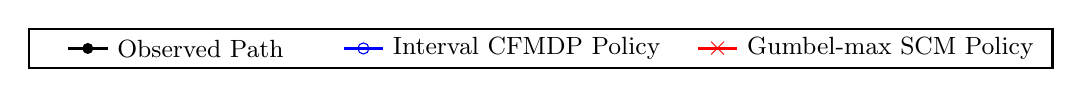
\begin{tikzpicture}[scale=1.0, every node/.style={scale=1.0}]
            \draw[thick, black] (-3, -0.25) rectangle (10, 0.25);
            %
            \draw[black, line width=1pt] (-2.5, 0.0) -- (-2,0.0);
            \fill[black] (-2.25,0.0) circle (2pt); %
            \node[right] at (-2,0.0) {\small Observed Path};
            
            %
            \draw[blue, line width=1pt] (1.0,0.0) -- (1.5,0.0);
            \node[draw=blue, circle, minimum size=4pt, inner sep=0pt] at (1.25,0.0) {}; %
            \node[right] at (1.5,0.0) {\small Interval CFMDP Policy};
            
            %
            \draw[red, line width=1pt] (5.5,0) -- (6,0);
            \node[red] at (5.75,0) {$\boldsymbol{\times}$}; %
            \node[right] at (6,0) {\small Gumbel-max SCM Policy};
        \end{tikzpicture}
    }\\
    %
    \subfigure[\footnotesize Lowest cumulative reward: Interval CFMDP ($312$), Gumbel-max SCM ($312$)]{%
        \resizebox{0.76\columnwidth}{!}{
             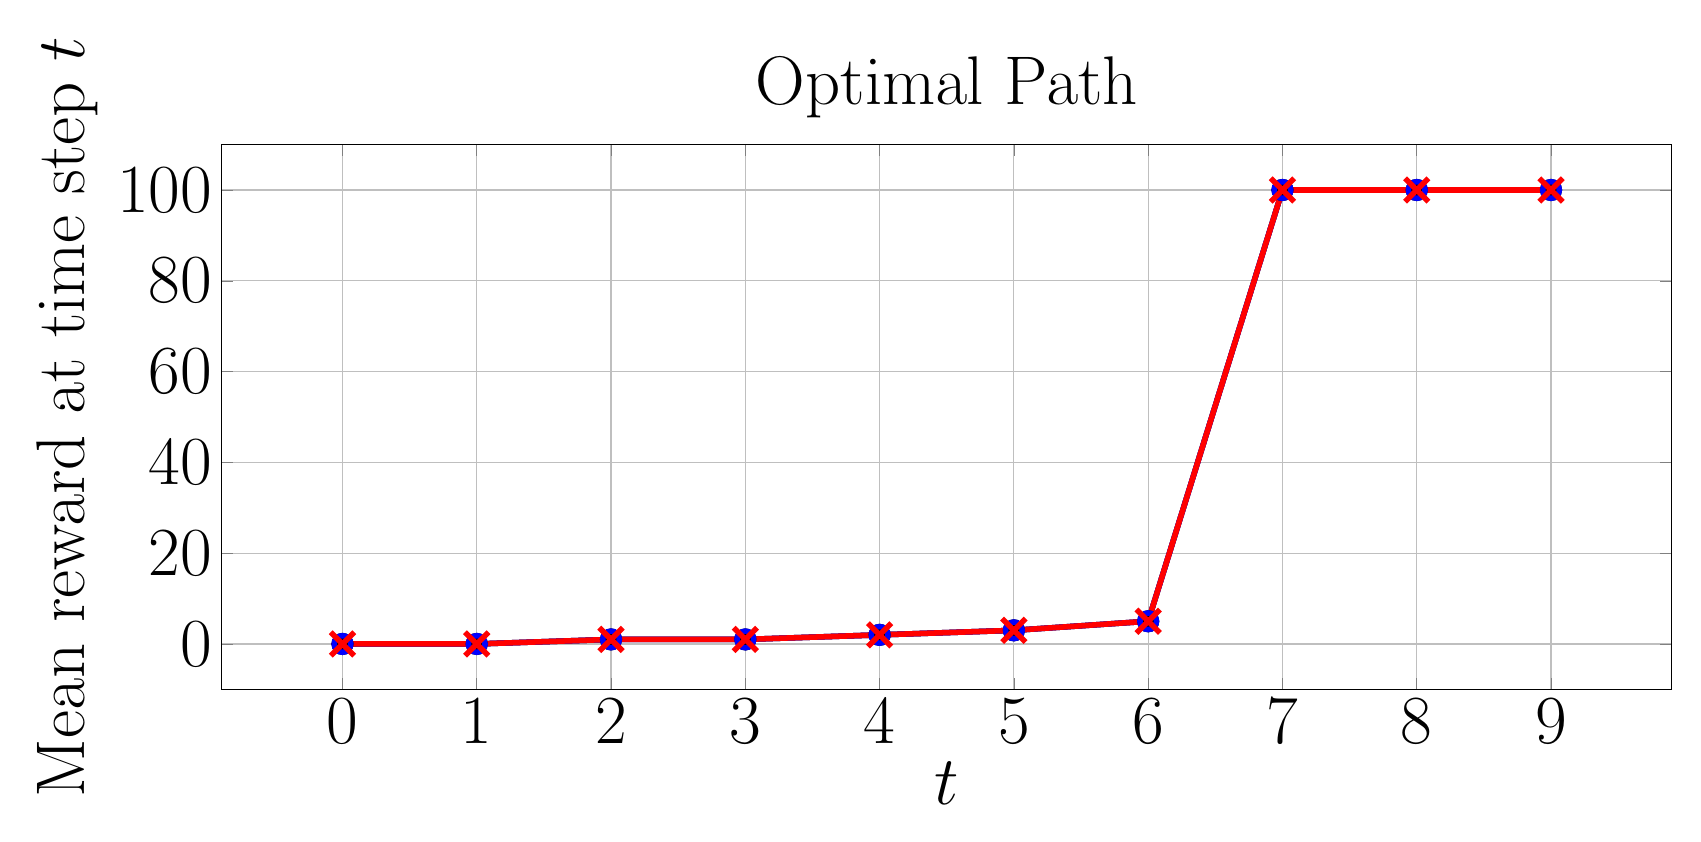
\begin{tikzpicture}
                \begin{axis}[
                    xlabel={$t$},
                    ylabel={Mean reward at time step $t$},
                    title={Optimal Path},
                    grid=both,
                    width=20cm, height=8.5cm,
                    every axis/.style={font=\Huge},
                    %
                ]
                \addplot[
                    color=black, %
                    mark=*, %
                    line width=2pt,
                    mark size=3pt,
                    error bars/.cd,
                    y dir=both, %
                    y explicit, %
                    error bar style={line width=1pt,solid},
                    error mark options={line width=1pt,mark size=4pt,rotate=90}
                ]
                coordinates {
                    (0, 0.0)  +- (0, 0.0)
                    (1, 0.0)  +- (0, 0.0) 
                    (2, 1.0)  +- (0, 0.0) 
                    (3, 1.0)  +- (0, 0.0)
                    (4, 2.0)  +- (0, 0.0)
                    (5, 3.0) +- (0, 0.0)
                    (6, 5.0) +- (0, 0.0)
                    (7, 100.0) +- (0, 0.0)
                    (8, 100.0) +- (0, 0.0)
                    (9, 100.0) +- (0, 0.0)
                };
                %
                \addplot[
                    color=blue, %
                    mark=o, %
                    line width=2pt,
                    mark size=3pt,
                    error bars/.cd,
                    y dir=both, %
                    y explicit, %
                    error bar style={line width=1pt,solid},
                    error mark options={line width=1pt,mark size=4pt,rotate=90}
                ]
                 coordinates {
                    (0, 0.0)  +- (0, 0.0)
                    (1, 0.0)  +- (0, 0.0) 
                    (2, 1.0)  +- (0, 0.0) 
                    (3, 1.0)  +- (0, 0.0)
                    (4, 2.0)  +- (0, 0.0)
                    (5, 3.0) +- (0, 0.0)
                    (6, 5.0) +- (0, 0.0)
                    (7, 100.0) +- (0, 0.0)
                    (8, 100.0) +- (0, 0.0)
                    (9, 100.0) +- (0, 0.0)
                };
                %
                \addplot[
                    color=red, %
                    mark=x, %
                    line width=2pt,
                    mark size=6pt,
                    error bars/.cd,
                    y dir=both, %
                    y explicit, %
                    error bar style={line width=1pt,solid},
                    error mark options={line width=1pt,mark size=4pt,rotate=90}
                ]
                coordinates {
                    (0, 0.0)  +- (0, 0.0)
                    (1, 0.0)  +- (0, 0.0) 
                    (2, 1.0)  +- (0, 0.0) 
                    (3, 1.0)  +- (0, 0.0)
                    (4, 2.0)  +- (0, 0.0)
                    (5, 3.0) +- (0, 0.0)
                    (6, 5.0) +- (0, 0.0)
                    (7, 100.0) +- (0, 0.0)
                    (8, 100.0) +- (0, 0.0)
                    (9, 100.0) +- (0, 0.0)
                };
                \end{axis}
            \end{tikzpicture}
         }
    }
    \hspace{1cm}
    \subfigure[\footnotesize Lowest cumulative reward: Interval CFMDP ($19$), Gumbel-max SCM ($-88$)]{%
         \resizebox{0.76\columnwidth}{!}{
            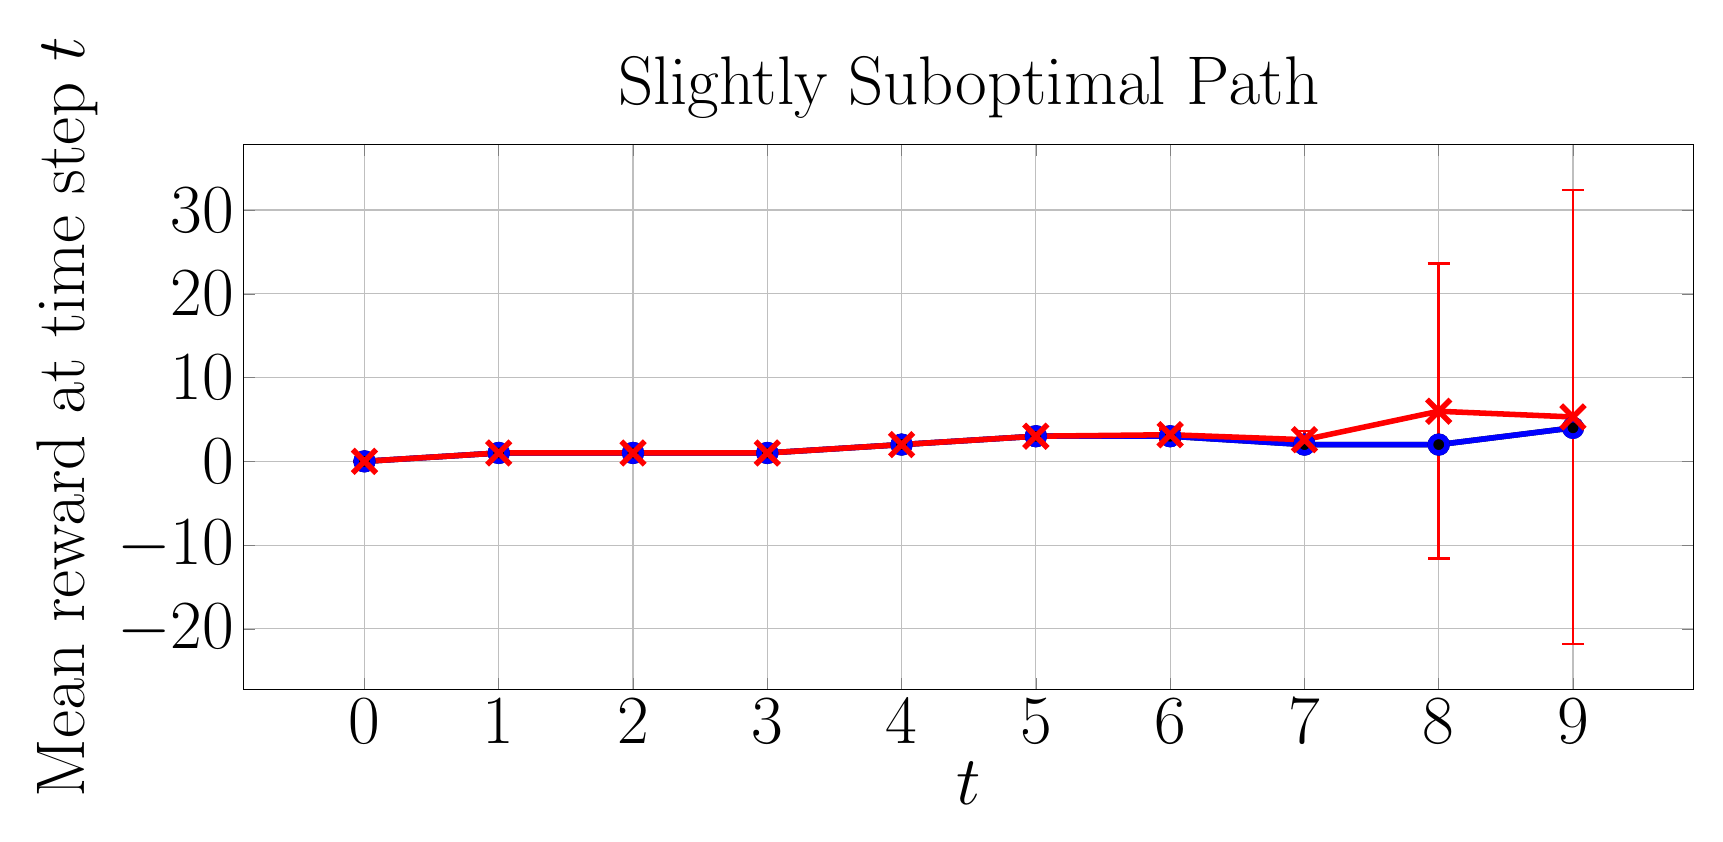
\begin{tikzpicture}
                \begin{axis}[
                    xlabel={$t$},
                    ylabel={Mean reward at time step $t$},
                    title={Slightly Suboptimal Path},
                    grid=both,
                    width=20cm, height=8.5cm,
                    every axis/.style={font=\Huge},
                    %
                ]
                \addplot[
                    color=black, %
                    mark=*, %
                    line width=2pt,
                    mark size=3pt,
                    error bars/.cd,
                    y dir=both, %
                    y explicit, %
                    error bar style={line width=1pt,solid},
                    error mark options={line width=1pt,mark size=4pt,rotate=90}
                ]
              coordinates {
                    (0, 0.0)  +- (0, 0.0)
                    (1, 1.0)  +- (0, 0.0) 
                    (2, 1.0)  +- (0, 0.0) 
                    (3, 1.0)  +- (0, 0.0)
                    (4, 2.0)  +- (0, 0.0)
                    (5, 3.0) +- (0, 0.0)
                    (6, 3.0) +- (0, 0.0)
                    (7, 2.0) +- (0, 0.0)
                    (8, 2.0) +- (0, 0.0)
                    (9, 4.0) +- (0, 0.0)
                };
                %
                \addplot[
                    color=blue, %
                    mark=o, %
                    line width=2pt,
                    mark size=3pt,
                    error bars/.cd,
                    y dir=both, %
                    y explicit, %
                    error bar style={line width=1pt,solid},
                    error mark options={line width=1pt,mark size=4pt,rotate=90}
                ]
              coordinates {
                    (0, 0.0)  +- (0, 0.0)
                    (1, 1.0)  +- (0, 0.0) 
                    (2, 1.0)  +- (0, 0.0) 
                    (3, 1.0)  +- (0, 0.0)
                    (4, 2.0)  +- (0, 0.0)
                    (5, 3.0) +- (0, 0.0)
                    (6, 3.0) +- (0, 0.0)
                    (7, 2.0) +- (0, 0.0)
                    (8, 2.0) +- (0, 0.0)
                    (9, 4.0) +- (0, 0.0)
                };
                %
                \addplot[
                    color=red, %
                    mark=x, %
                    line width=2pt,
                    mark size=6pt,
                    error bars/.cd,
                    y dir=both, %
                    y explicit, %
                    error bar style={line width=1pt,solid},
                    error mark options={line width=1pt,mark size=4pt,rotate=90}
                ]
                coordinates {
                    (0, 0.0)  +- (0, 0.0)
                    (1, 1.0)  +- (0, 0.0) 
                    (2, 1.0)  +- (0, 0.0) 
                    (3, 1.0)  +- (0, 0.0)
                    (4, 2.0)  += (0, 0.0)
                    (5, 3.0)  += (0, 0.0)
                    (6, 3.17847) += (0, 0.62606746) -= (0, 0.62606746)
                    (7, 2.5832885) += (0, 1.04598233) -= (0, 1.04598233)
                    (8, 5.978909) += (0, 17.60137623) -= (0, 17.60137623)
                    (9, 5.297059) += (0, 27.09227512) -= (0, 27.09227512)
                };
                \end{axis}
            \end{tikzpicture}
         }
    }\\[-1.5pt]
    \subfigure[\footnotesize Lowest cumulative reward: Interval CFMDP ($14$), Gumbel-max SCM ($-598$)]{%
         \resizebox{0.76\columnwidth}{!}{
             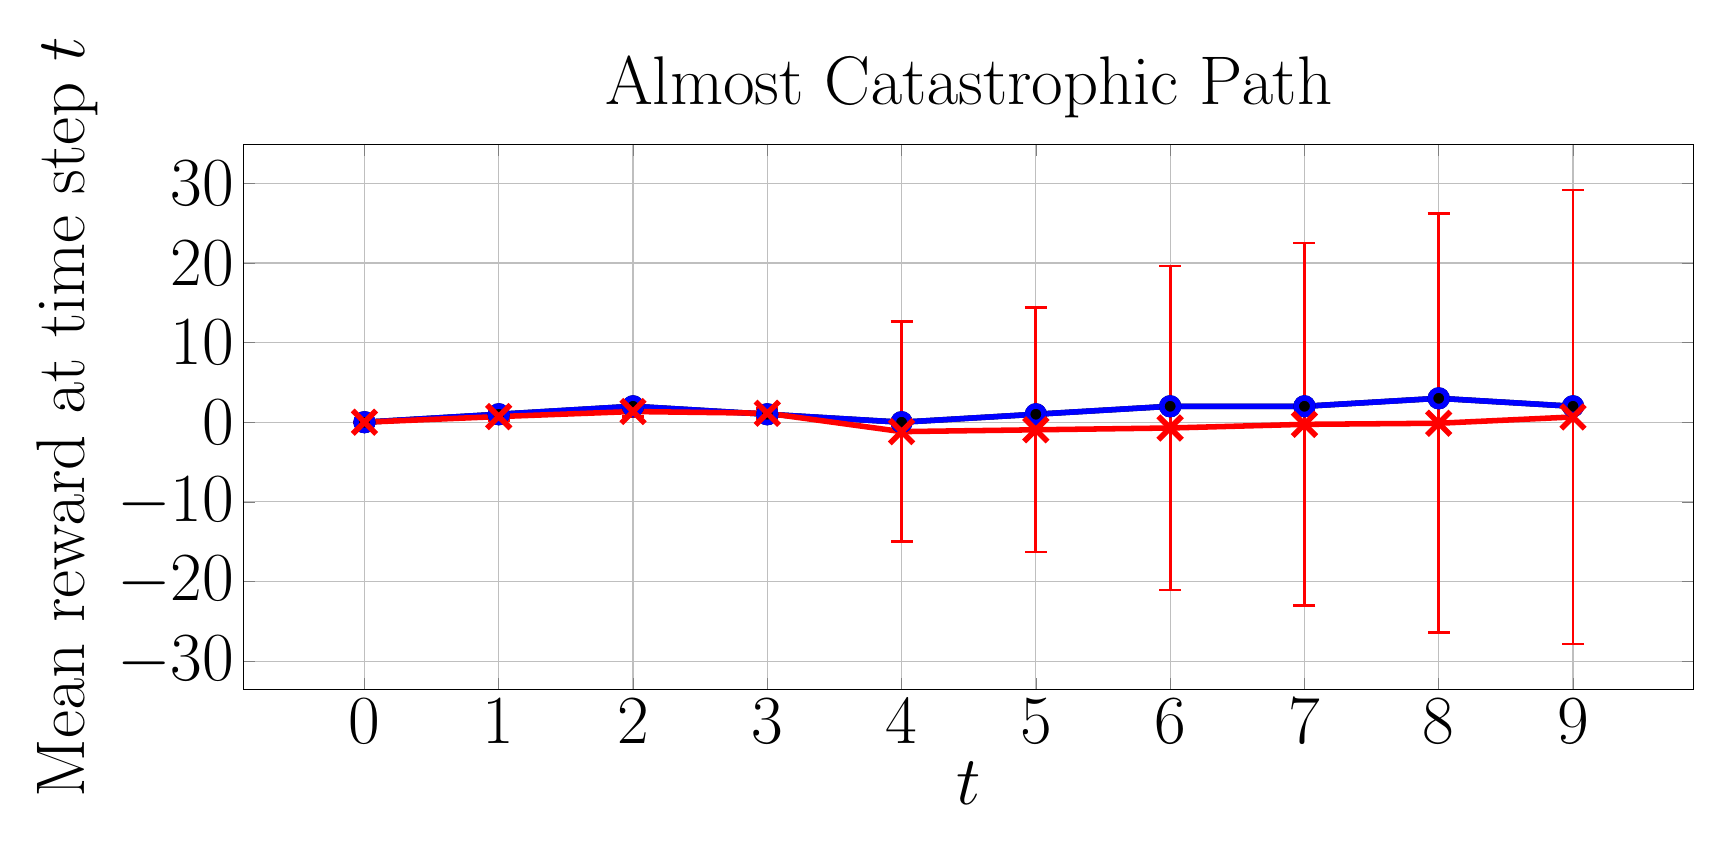
\begin{tikzpicture}
                \begin{axis}[
                    xlabel={$t$},
                    ylabel={Mean reward at time step $t$},
                    title={Almost Catastrophic Path},
                    grid=both,
                    width=20cm, height=8.5cm,
                    every axis/.style={font=\Huge},
                    %
                ]
                \addplot[
                    color=black, %
                    mark=*, %
                    line width=2pt,
                    mark size=3pt,
                    error bars/.cd,
                    y dir=both, %
                    y explicit, %
                    error bar style={line width=1pt,solid},
                    error mark options={line width=1pt,mark size=4pt,rotate=90}
                ]
                coordinates {
                    (0, 0.0)  +- (0, 0.0)
                    (1, 1.0)  +- (0, 0.0) 
                    (2, 2.0)  +- (0, 0.0) 
                    (3, 1.0)  +- (0, 0.0)
                    (4, 0.0)  +- (0, 0.0)
                    (5, 1.0) +- (0, 0.0)
                    (6, 2.0) +- (0, 0.0)
                    (7, 2.0) +- (0, 0.0)
                    (8, 3.0) +- (0, 0.0)
                    (9, 2.0) +- (0, 0.0)
                };
                %
                \addplot[
                    color=blue, %
                    mark=o, %
                    line width=2pt,
                    mark size=3pt,
                    error bars/.cd,
                    y dir=both, %
                    y explicit, %
                    error bar style={line width=1pt,solid},
                    error mark options={line width=1pt,mark size=4pt,rotate=90}
                ]
                coordinates {
                    (0, 0.0)  +- (0, 0.0)
                    (1, 1.0)  +- (0, 0.0) 
                    (2, 2.0)  +- (0, 0.0) 
                    (3, 1.0)  +- (0, 0.0)
                    (4, 0.0)  +- (0, 0.0)
                    (5, 1.0) +- (0, 0.0)
                    (6, 2.0) +- (0, 0.0)
                    (7, 2.0) +- (0, 0.0)
                    (8, 3.0) +- (0, 0.0)
                    (9, 2.0) +- (0, 0.0)
                };
                %
                \addplot[
                    color=red, %
                    mark=x, %
                    line width=2pt,
                    mark size=6pt,
                    error bars/.cd,
                    y dir=both, %
                    y explicit, %
                    error bar style={line width=1pt,solid},
                    error mark options={line width=1pt,mark size=4pt,rotate=90}
                ]
                coordinates {
                    (0, 0.0)  +- (0, 0.0)
                    (1, 0.7065655)  +- (0, 0.4553358) 
                    (2, 1.341673)  +- (0, 0.67091621) 
                    (3, 1.122926)  +- (0, 0.61281824)
                    (4, -1.1821935)  +- (0, 13.82444042)
                    (5, -0.952399)  +- (0, 15.35195457)
                    (6, -0.72672) +- (0, 20.33508414)
                    (7, -0.268983) +- (0, 22.77861454)
                    (8, -0.1310835) +- (0, 26.31013314)
                    (9, 0.65806) +- (0, 28.50670214)
                };
                %
            %
            %
            %
            %
            %
            %
            %
            %
            %
            %
            %
            %
            %
            %
            %
            %
            %
            %
                \end{axis}
            \end{tikzpicture}
         }
    }
    \hspace{1cm}
    \subfigure[\footnotesize Lowest cumulative reward: Interval CFMDP ($-698$), Gumbel-max SCM ($-698$)]{%
         \resizebox{0.76\columnwidth}{!}{
            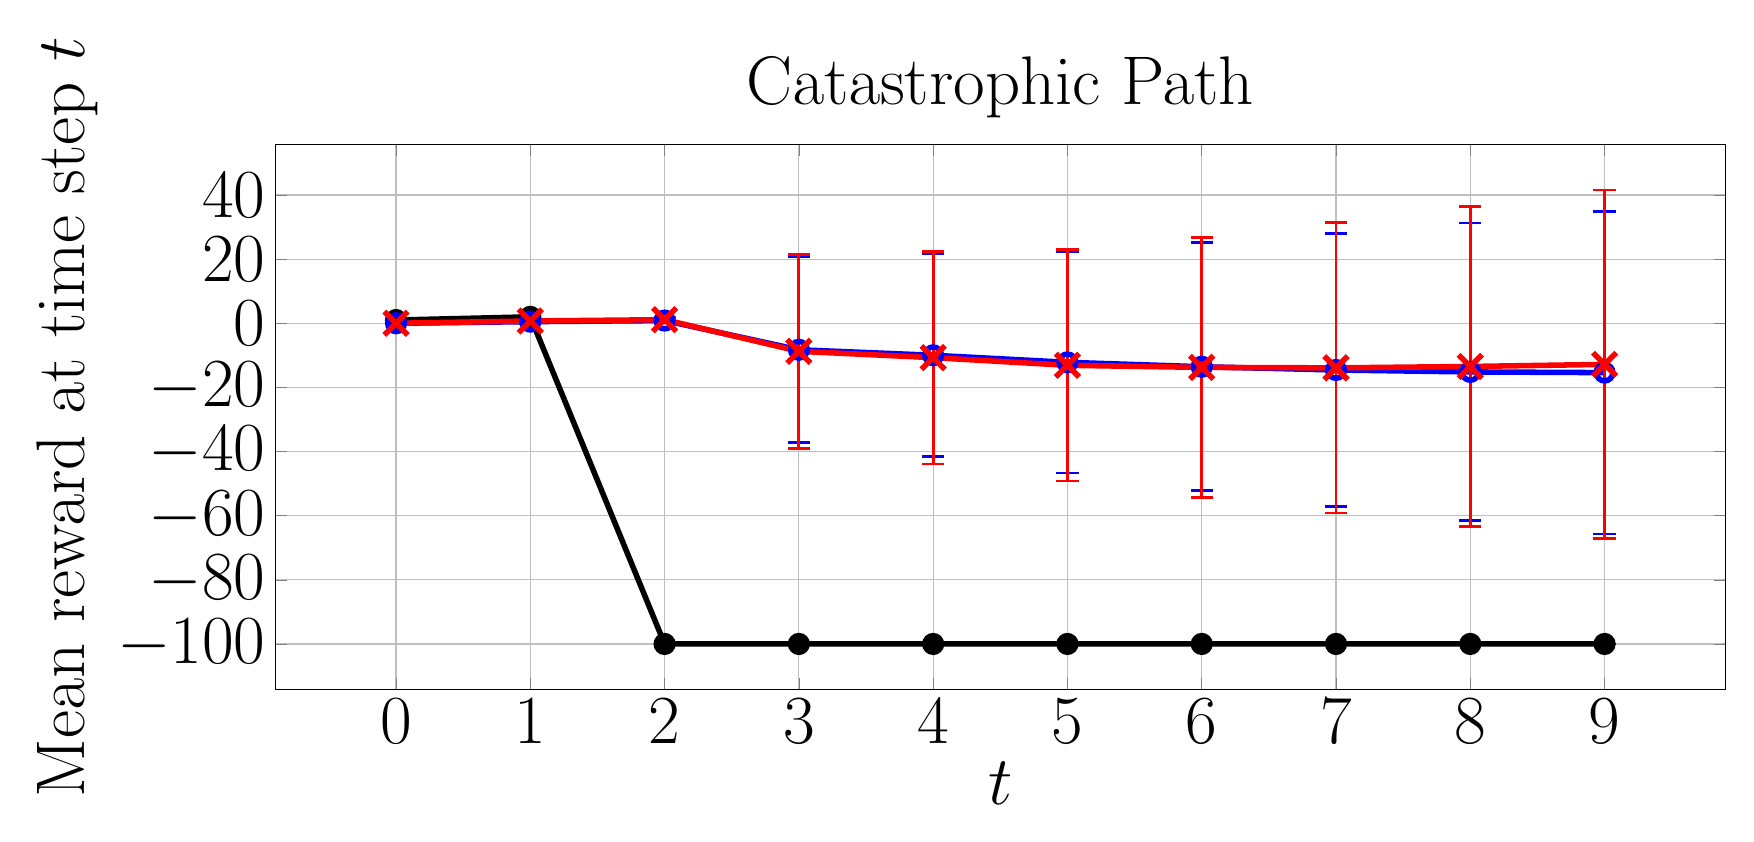
\begin{tikzpicture}
                \begin{axis}[
                    xlabel={$t$},
                    ylabel={Mean reward at time step $t$},
                    title={Catastrophic Path},
                    grid=both,
                    width=20cm, height=8.5cm,
                    every axis/.style={font=\Huge},
                    %
                ]
                \addplot[
                    color=black, %
                    mark=*, %
                    line width=2pt,
                    mark size=3pt,
                    error bars/.cd,
                    y dir=both, %
                    y explicit, %
                    error bar style={line width=1pt,solid},
                    error mark options={line width=1pt,mark size=4pt,rotate=90}
                ]
                coordinates {
                    (0, 1.0)  +- (0, 0.0)
                    (1, 2.0)  +- (0, 0.0) 
                    (2, -100.0)  +- (0, 0.0) 
                    (3, -100.0)  +- (0, 0.0)
                    (4, -100.0)  +- (0, 0.0)
                    (5, -100.0) +- (0, 0.0)
                    (6, -100.0) +- (0, 0.0)
                    (7, -100.0) +- (0, 0.0)
                    (8, -100.0) +- (0, 0.0)
                    (9, -100.0) +- (0, 0.0)
                };
                %
                \addplot[
                    color=blue, %
                    mark=o, %
                    line width=2pt,
                    mark size=3pt,
                    error bars/.cd,
                    y dir=both, %
                    y explicit, %
                    error bar style={line width=1pt,solid},
                    error mark options={line width=1pt,mark size=4pt,rotate=90}
                ]
                coordinates {
                    (0, 0.0)  +- (0, 0.0)
                    (1, 0.504814)  +- (0, 0.49997682) 
                    (2, 0.8439835)  +- (0, 0.76831917) 
                    (3, -8.2709165)  +- (0, 28.93656754)
                    (4, -9.981082)  +- (0, 31.66825363)
                    (5, -12.1776325) +- (0, 34.53463233)
                    (6, -13.556076) +- (0, 38.62845372)
                    (7, -14.574418) +- (0, 42.49603359)
                    (8, -15.1757075) +- (0, 46.41913968)
                    (9, -15.3900395) +- (0, 50.33563368)
                };
                %
                \addplot[
                    color=red, %
                    mark=x, %
                    line width=2pt,
                    mark size=6pt,
                    error bars/.cd,
                    y dir=both, %
                    y explicit, %
                    error bar style={line width=1pt,solid},
                    error mark options={line width=1pt,mark size=4pt,rotate=90}
                ]
                coordinates {
                    (0, 0.0)  +- (0, 0.0)
                    (1, 0.701873)  +- (0, 0.45743556) 
                    (2, 1.1227805)  +- (0, 0.73433129) 
                    (3, -8.7503255)  +- (0, 30.30257976)
                    (4, -10.722092)  +- (0, 33.17618589)
                    (5, -13.10721)  +- (0, 36.0648089)
                    (6, -13.7631645) +- (0, 40.56553451)
                    (7, -13.909043) +- (0, 45.23829402)
                    (8, -13.472517) +- (0, 49.96270296)
                    (9, -12.8278835) +- (0, 54.38618735)
                };
                %
            %
            %
            %
            %
            %
            %
            %
            %
            %
            %
            %
            %
            %
            %
            %
            %
            %
            %
                \end{axis}
            \end{tikzpicture}
         }
    }
    \caption{Average instant reward of CF paths induced by policies on GridWorld $p=0.4$.}
    \label{fig: reward p=0.4}
\end{figure*}

\subsection{Experimental Setup}
To compare policy performance, we measure the average rewards of counterfactual paths induced by our policy and the Gumbel-max policy by uniformly sampling $200$ counterfactual MDPs from the ICFMDP and generating $10,000$ counterfactual paths over each sampled CFMDP. \jl{Since the interval CFMDP depends on the observed path, we select $4$  paths of varying optimality to evaluate how the observed path impacts the performance of both policies: an optimal path, a slightly suboptimal path that could reach the optimal reward with a few changes, a catastrophic path that enters a catastrophic, terminal state with low reward, and an almost catastrophic path that was close to entering a catastrophic state.} When measuring the average probability bound widths and execution time needed to generate the ICFMDPs, we averaged over $20$ randomly generated observed paths
\footnote{Further training details are provided in Appendix \ref{app: training details}, and the code is provided at \href{https://github.com/ddv-lab/robust-cf-inference-in-MDPs}{https://github.com/ddv-lab/robust-cf-inference-in-MDPs}
%
%
.}.

\subsection{GridWorld}
\jl{The GridWorld MDP is a $4 \times 4$ grid where an agent must navigate from the top-left corner to the goal state in the bottom-right corner, avoiding a dangerous terminal state in the centre. At each time step, the agent can move up, down, left, or right, but there is a small probability (controlled by hyper-parameter $p$) of moving in an unintended direction. As the agent nears the goal, the reward for each state increases, culminating in a reward of $+100$ for reaching the goal. Entering the dangerous state results in a penalty of $-100$. We use two versions of GridWorld: a less stochastic version with $p=0.9$ (i.e., $90$\% chance of moving in the chosen direction) and a more stochastic version with $p=0.4$.}

\paragraph{GridWorld ($p=0.9$)}
When $p=0.9$, the counterfactual probability bounds are typically narrow (see Table \ref{tab:nonzero_probs} for average measurements). Consequently, as shown in Figure \ref{fig: reward p=0.9}, both policies are nearly identical and perform similarly well across the optimal, slightly suboptimal, and catastrophic paths.
%
However, for the almost catastrophic path, the interval CFMDP path is more conservative and follows the observed path more closely (as this is where the probability bounds are narrowest), which typically requires one additional step to reach the goal state than the Gumbel-max SCM policy.
%

\paragraph{GridWorld ($p=0.4$)}
\jl{When $p=0.4$, the GridWorld environment becomes more uncertain, increasing the risk of entering the dangerous state even if correct actions are chosen. Thus, as shown in Figure \ref{fig: reward p=0.4}, the interval CFMDP policy adopts a more conservative approach, avoiding deviation from the observed policy if it cannot guarantee higher counterfactual rewards (see the slightly suboptimal and almost catastrophic paths), whereas the Gumbel-max SCM is inconsistent: it can yield higher rewards, but also much lower rewards, reflected in the wide error bars.} For the catastrophic path, both policies must deviate from the observed path to achieve a higher reward and, in this case, perform similarly.
%
%
%
%
\subsection{Sepsis}
The Sepsis MDP \citep{oberst2019counterfactual} simulates trajectories of Sepsis patients. Each state consists of four vital signs (heart rate, blood pressure, oxygen concentration, and glucose levels), categorised as low, normal, or high.
and three treatments that can be toggled on/off at each time step (8 actions in total). Unlike \citet{oberst2019counterfactual}, we scale rewards based on the number of out-of-range vital signs, between $-1000$ (patient dies) and $1000$ (patient discharged). \jl{Like the GridWorld $p=0.4$ experiment, the Sepsis MDP is highly uncertain, as many states are equally likely to lead to optimal and poor outcomes. Thus, as shown in Figure \ref{fig: reward sepsis}, both policies follow the observed optimal and almost catastrophic paths to guarantee rewards are no worse than the observation.} However, improving the catastrophic path requires deviating from the observation. Here, the Gumbel-max SCM policy, on average, performs better than the interval CFMDP policy. But, since both policies have lower bounds clipped at $-1000$, neither policy reliably improves over the observation. In contrast, for the slightly suboptimal path, the interval CFMDP policy performs significantly better, shown by its higher lower bounds. 
Moreover, in these two cases, the worst-case counterfactual path generated by the interval CFMDP policy is better than that of the Gumbel-max SCM policy,
indicating its greater robustness.
%
\begin{figure*}
    \centering
     \resizebox{0.6\textwidth}{!}{
        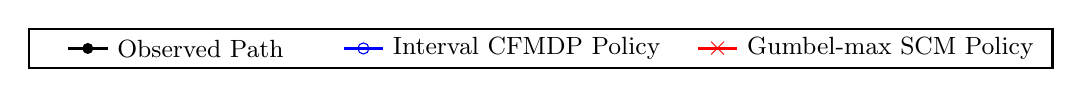
\begin{tikzpicture}[scale=1.0, every node/.style={scale=1.0}]
            \draw[thick, black] (-3, -0.25) rectangle (10, 0.25);
            %
            \draw[black, line width=1pt] (-2.5, 0.0) -- (-2,0.0);
            \fill[black] (-2.25,0.0) circle (2pt); %
            \node[right] at (-2,0.0) {\small Observed Path};
            
            %
            \draw[blue, line width=1pt] (1.0,0.0) -- (1.5,0.0);
            \node[draw=blue, circle, minimum size=4pt, inner sep=0pt] at (1.25,0.0) {}; %
            \node[right] at (1.5,0.0) {\small Interval CFMDP Policy};
            
            %
            \draw[red, line width=1pt] (5.5,0) -- (6,0);
            \node[red] at (5.75,0) {$\boldsymbol{\times}$}; %
            \node[right] at (6,0) {\small Gumbel-max SCM Policy};
        \end{tikzpicture}
    }\\
    \subfigure[\footnotesize Lowest cumulative reward: Interval CFMDP ($8000$), Gumbel-max SCM ($8000$)]{%
         \resizebox{0.76\columnwidth}{!}{
             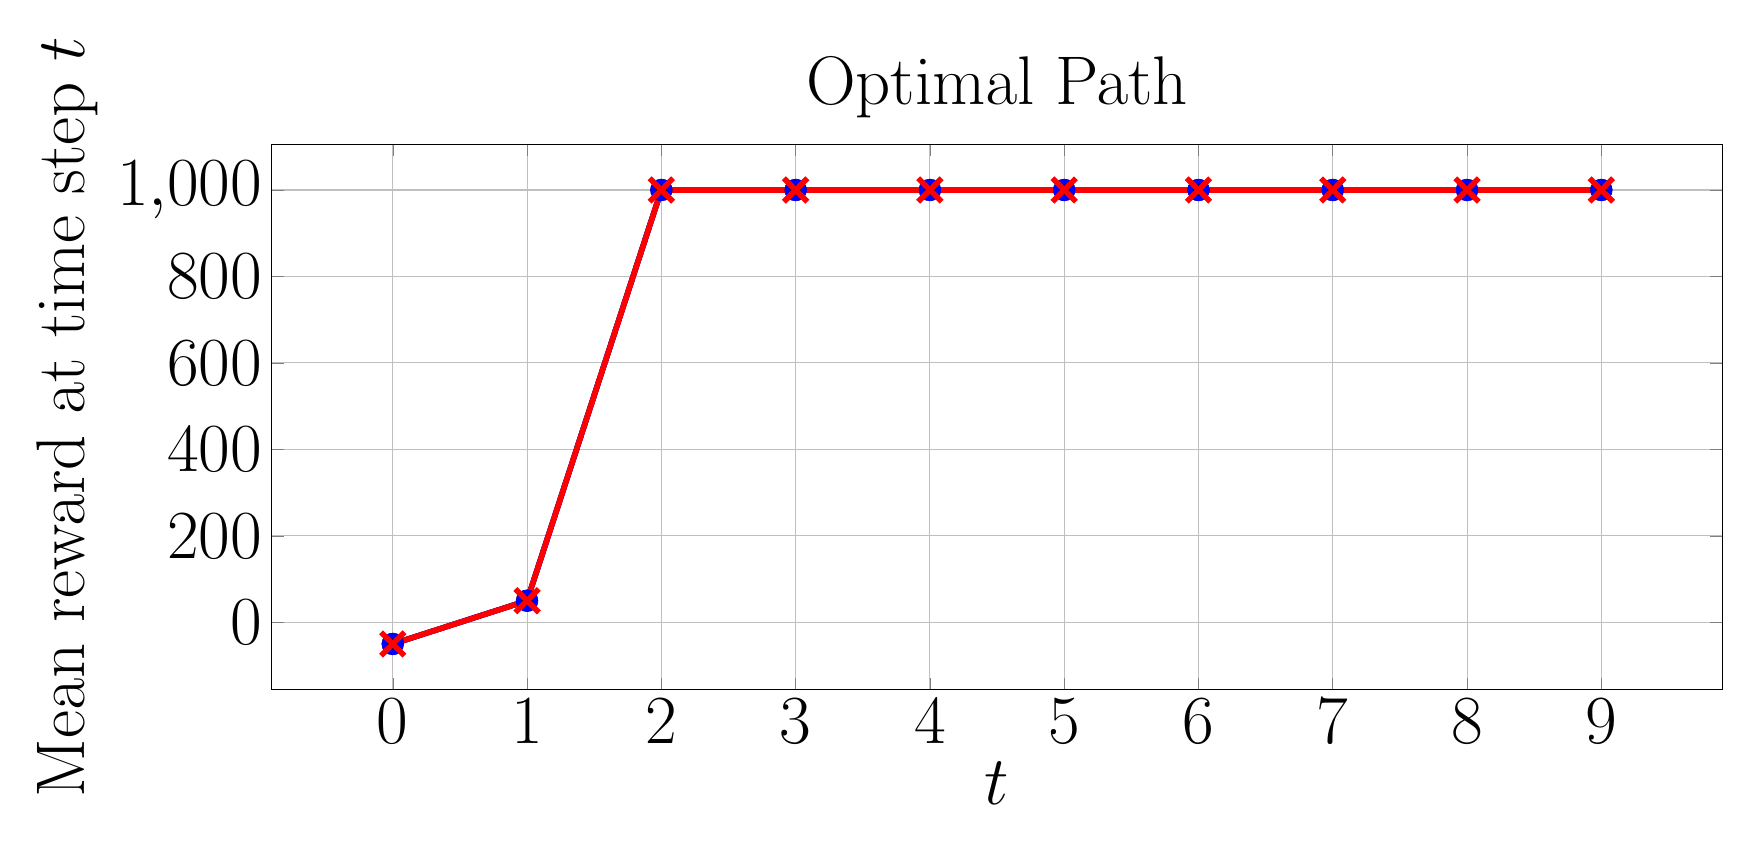
\begin{tikzpicture}
                \begin{axis}[
                    xlabel={$t$},
                    ylabel={Mean reward at time step $t$},
                    title={Optimal Path},
                    grid=both,
                    width=20cm, height=8.5cm,
                    every axis/.style={font=\Huge},
                    %
                ]
                \addplot[
                    color=black, %
                    mark=*, %
                    line width=2pt,
                    mark size=3pt,
                ]
                coordinates {
                    (0, -50.0)
                    (1, 50.0)
                    (2, 1000.0)
                    (3, 1000.0)
                    (4, 1000.0)
                    (5, 1000.0)
                    (6, 1000.0)
                    (7, 1000.0)
                    (8, 1000.0)
                    (9, 1000.0)
                };
                %
                \addplot[
                    color=blue, %
                    mark=o, %
                    line width=2pt,
                    mark size=3pt,
                    error bars/.cd,
                    y dir=both, %
                    y explicit, %
                    error bar style={line width=1pt,solid},
                    error mark options={line width=1pt,mark size=4pt,rotate=90}
                ]
                coordinates {
                    (0, -50.0)  +- (0, 0.0)
                    (1, 50.0)  +- (0, 0.0) 
                    (2, 1000.0)  +- (0, 0.0) 
                    (3, 1000.0)  +- (0, 0.0)
                    (4, 1000.0)  +- (0, 0.0)
                    (5, 1000.0) +- (0, 0.0)
                    (6, 1000.0) +- (0, 0.0)
                    (7, 1000.0) +- (0, 0.0)
                    (8, 1000.0) +- (0, 0.0)
                    (9, 1000.0) +- (0, 0.0)
                };
                %
                \addplot[
                    color=red, %
                    mark=x, %
                    line width=2pt,
                    mark size=6pt,
                    error bars/.cd,
                    y dir=both, %
                    y explicit, %
                    error bar style={line width=1pt,solid},
                    error mark options={line width=1pt,mark size=4pt,rotate=90}
                ]
                coordinates {
                    (0, -50.0)  +- (0, 0.0)
                    (1, 50.0)  +- (0, 0.0) 
                    (2, 1000.0)  +- (0, 0.0) 
                    (3, 1000.0)  +- (0, 0.0)
                    (4, 1000.0)  +- (0, 0.0)
                    (5, 1000.0) +- (0, 0.0)
                    (6, 1000.0) +- (0, 0.0)
                    (7, 1000.0) +- (0, 0.0)
                    (8, 1000.0) +- (0, 0.0)
                    (9, 1000.0) +- (0, 0.0)
                };
                %
                \end{axis}
            \end{tikzpicture}
         }
    }
    \hspace{1cm}
    \subfigure[\footnotesize Lowest cumulative reward: Interval CFMDP ($-5980$), Gumbel-max SCM ($-8000$)]{%
         \resizebox{0.76\columnwidth}{!}{
            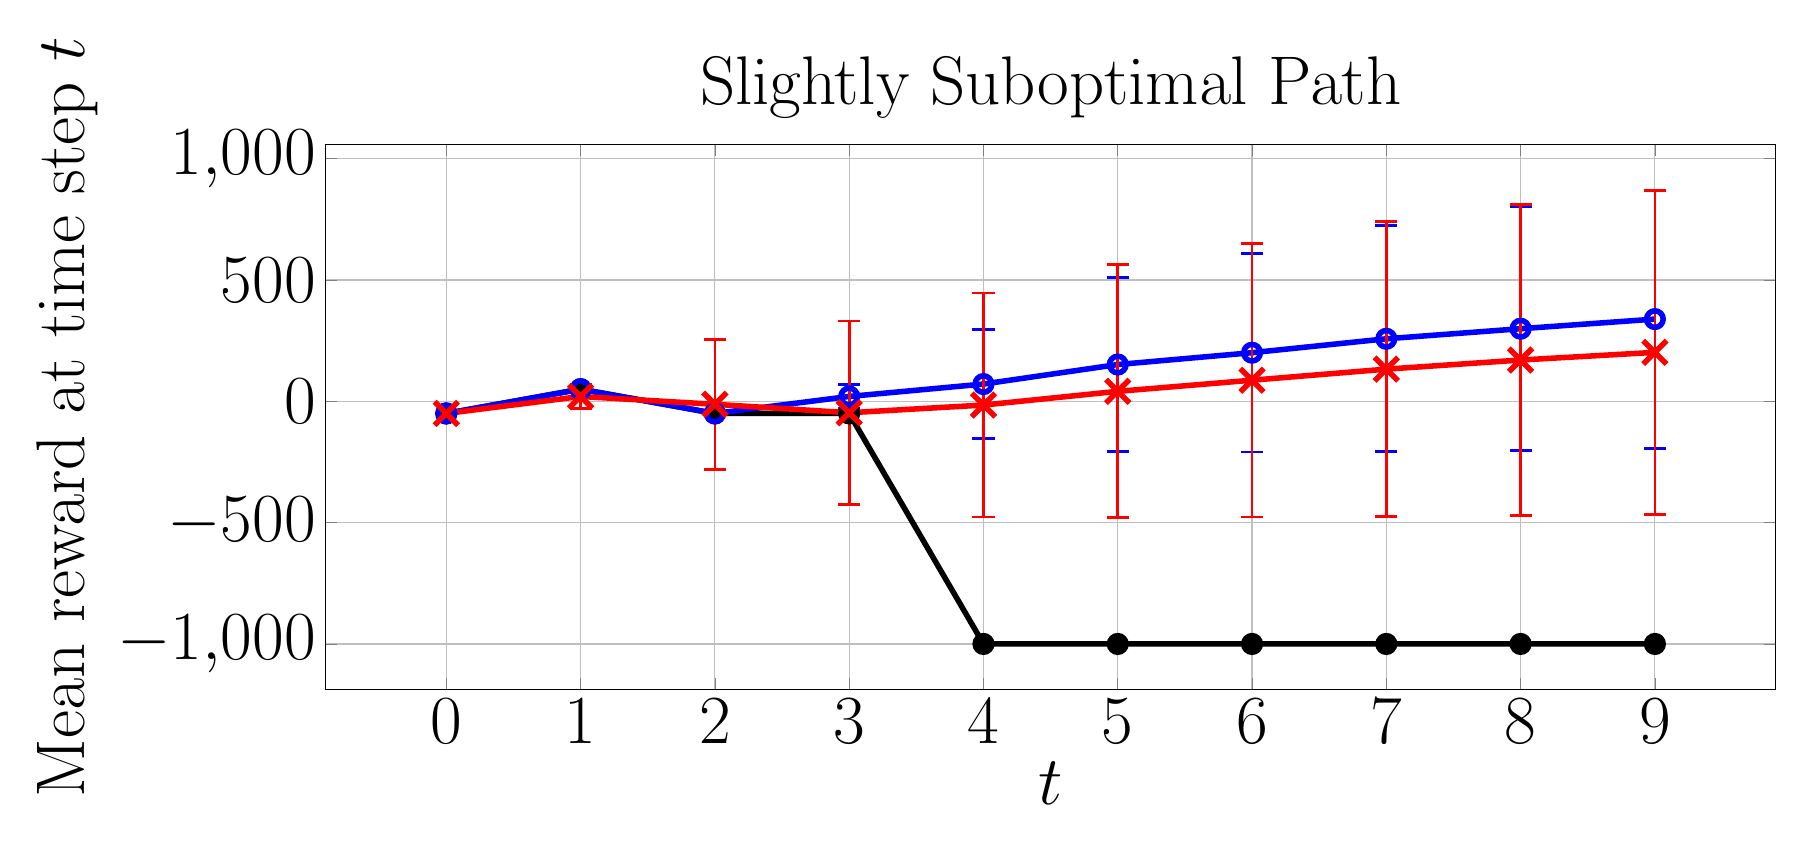
\begin{tikzpicture}
                \begin{axis}[
                    xlabel={$t$},
                    ylabel={Mean reward at time step $t$},
                    title={Slightly Suboptimal Path},
                    grid=both,
                    width=20cm, height=8.5cm,
                    every axis/.style={font=\Huge},
                    %
                ]
               \addplot[
                    color=black, %
                    mark=*, %
                    line width=2pt,
                    mark size=3pt,
                ]
                coordinates {
                    (0, -50.0)
                    (1, 50.0)
                    (2, -50.0)
                    (3, -50.0)
                    (4, -1000.0)
                    (5, -1000.0)
                    (6, -1000.0)
                    (7, -1000.0)
                    (8, -1000.0)
                    (9, -1000.0)
                };
                %
                \addplot[
                    color=blue, %
                    mark=o, %
                    line width=2pt,
                    mark size=3pt,
                    error bars/.cd,
                    y dir=both, %
                    y explicit, %
                    error bar style={line width=1pt,solid},
                    error mark options={line width=1pt,mark size=4pt,rotate=90}
                ]
                coordinates {
                    (0, -50.0)  +- (0, 0.0)
                    (1, 50.0)  +- (0, 0.0) 
                    (2, -50.0)  +- (0, 0.0) 
                    (3, 20.0631)  +- (0, 49.97539413)
                    (4, 71.206585)  +- (0, 226.02033693)
                    (5, 151.60797) +- (0, 359.23292559)
                    (6, 200.40593) +- (0, 408.86185176)
                    (7, 257.77948) +- (0, 466.10372804)
                    (8, 299.237465) +- (0, 501.82579506)
                    (9, 338.9129) +- (0, 532.06124996)
                };
                %
                \addplot[
                    color=red, %
                    mark=x, %
                    line width=2pt,
                    mark size=6pt,
                    error bars/.cd,
                    y dir=both, %
                    y explicit, %
                    error bar style={line width=1pt,solid},
                    error mark options={line width=1pt,mark size=4pt,rotate=90}
                ]
                coordinates {
                    (0, -50.0)  +- (0, 0.0)
                    (1, 20.00736)  +- (0, 49.99786741) 
                    (2, -12.282865)  +- (0, 267.598755) 
                    (3, -47.125995)  +- (0, 378.41755832)
                    (4, -15.381965)  +- (0, 461.77616558)
                    (5, 41.15459) +- (0, 521.53189262)
                    (6, 87.01595) +- (0, 564.22243126 )
                    (7, 132.62376) +- (0, 607.31338037)
                    (8, 170.168145) +- (0, 641.48013693)
                    (9, 201.813135) +- (0, 667.29441777)
                };
                %
                %
                %
                %
                %
                %
                %
                %
                %
                %
                %
                %
                %
                %
                %
                %
                %
                %
                %
                \end{axis}
            \end{tikzpicture}
         }
    }\\[-1.5pt]
    \subfigure[\footnotesize Lowest cumulative reward: Interval CFMDP ($100$), Gumbel-max SCM ($100$)]{%
         \resizebox{0.76\columnwidth}{!}{
             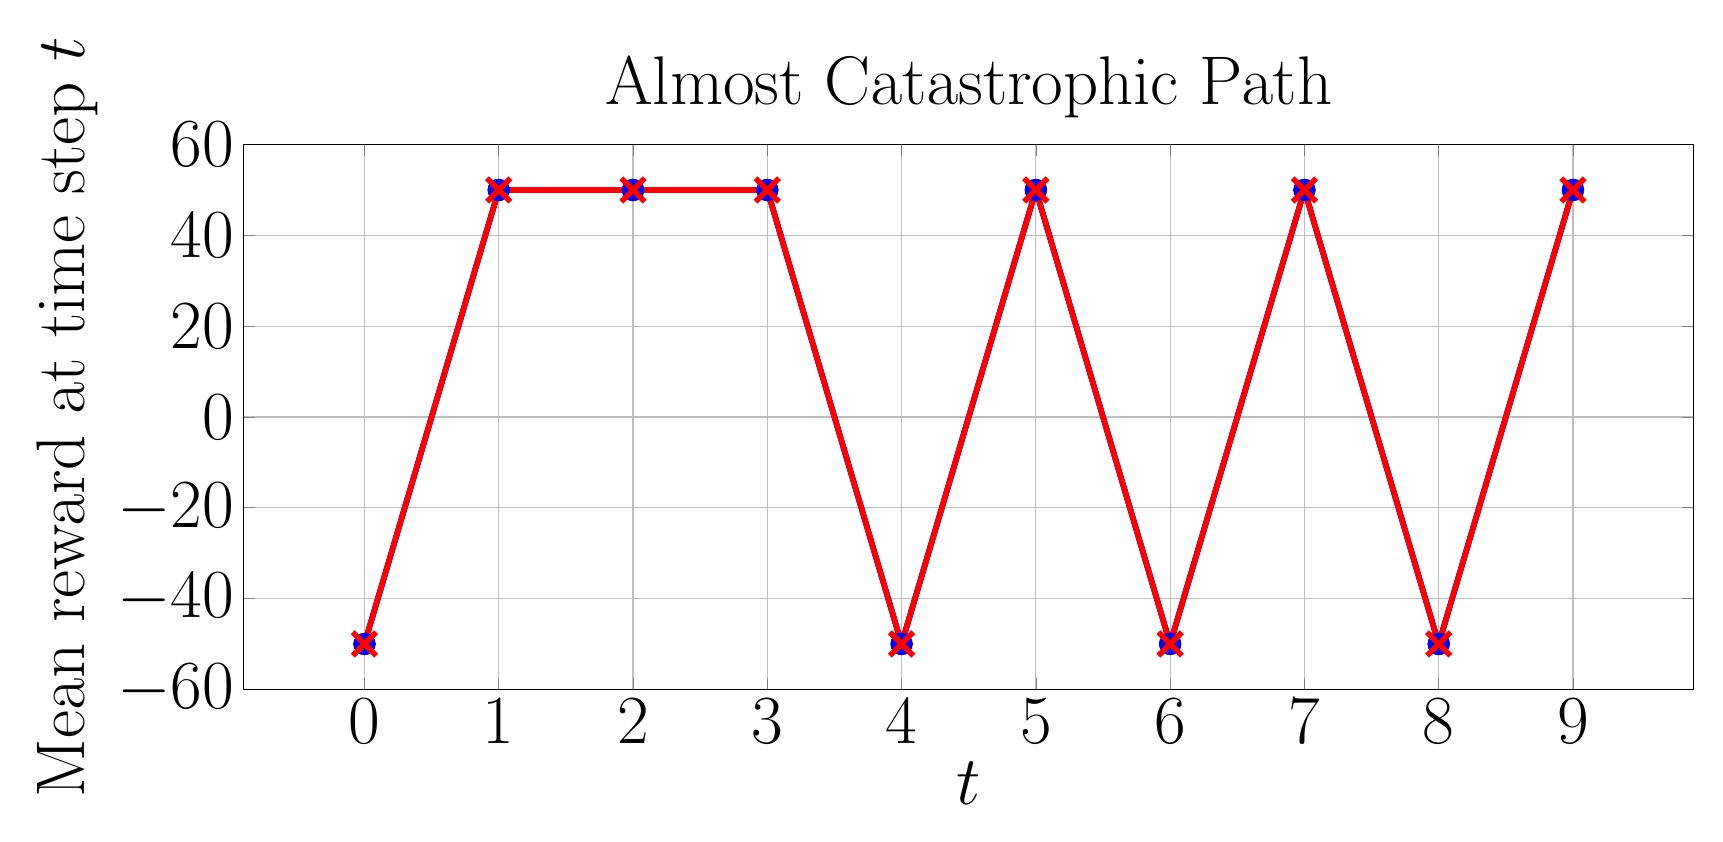
\begin{tikzpicture}
                \begin{axis}[
                    xlabel={$t$},
                    ylabel={Mean reward at time step $t$},
                    title={Almost Catastrophic Path},
                    grid=both,
                    every axis/.style={font=\Huge},
                    width=20cm, height=8.5cm,
                    %
                ]
               \addplot[
                    color=black, %
                    mark=*, %
                    line width=2pt,
                    mark size=3pt,
                ]
                coordinates {
                    (0, -50.0)
                    (1, 50.0)
                    (2, 50.0)
                    (3, 50.0)
                    (4, -50.0)
                    (5, 50.0)
                    (6, -50.0)
                    (7, 50.0)
                    (8, -50.0)
                    (9, 50.0)
                };
                %
                %
                \addplot[
                    color=blue, %
                    mark=o, %
                    line width=2pt,
                    mark size=3pt,
                    error bars/.cd,
                    y dir=both, %
                    y explicit, %
                    error bar style={line width=1pt,solid},
                    error mark options={line width=1pt,mark size=4pt,rotate=90}
                ]
                coordinates {
                    (0, -50.0)  +- (0, 0.0)
                    (1, 50.0)  +- (0, 0.0) 
                    (2, 50.0)  +- (0, 0.0) 
                    (3, 50.0)  +- (0, 0.0)
                    (4, -50.0)  +- (0, 0.0)
                    (5, 50.0) +- (0, 0.0)
                    (6, -50.0) +- (0, 0.0)
                    (7, 50.0) +- (0, 0.0)
                    (8, -50.0) +- (0, 0.0)
                    (9, 50.0) +- (0, 0.0)
                };
                %
                \addplot[
                    color=red, %
                    mark=x, %
                    line width=2pt,
                    mark size=6pt,
                    error bars/.cd,
                    y dir=both, %
                    y explicit, %
                    error bar style={line width=1pt,solid},
                    error mark options={line width=1pt,mark size=4pt,rotate=90}
                ]
                coordinates {
                    (0, -50.0)  +- (0, 0.0)
                    (1, 50.0)  +- (0, 0.0) 
                    (2, 50.0)  +- (0, 0.0) 
                    (3, 50.0)  +- (0, 0.0)
                    (4, -50.0)  +- (0, 0.0)
                    (5, 50.0) +- (0, 0.0)
                    (6, -50.0) +- (0, 0.0)
                    (7, 50.0) +- (0, 0.0)
                    (8, -50.0) +- (0, 0.0)
                    (9, 50.0) +- (0, 0.0)
                };
                %
                %
                %
                %
                %
                %
                %
                %
                %
                %
                %
                %
                %
                %
                %
                %
                %
                %
                %
                \end{axis}
            \end{tikzpicture}
         }
    }
    \hspace{1cm}
    \subfigure[\footnotesize Lowest cumulative reward: Interval CFMDP ($-7150$), Gumbel-max SCM ($-9050$)]{%
         \resizebox{0.76\columnwidth}{!}{
            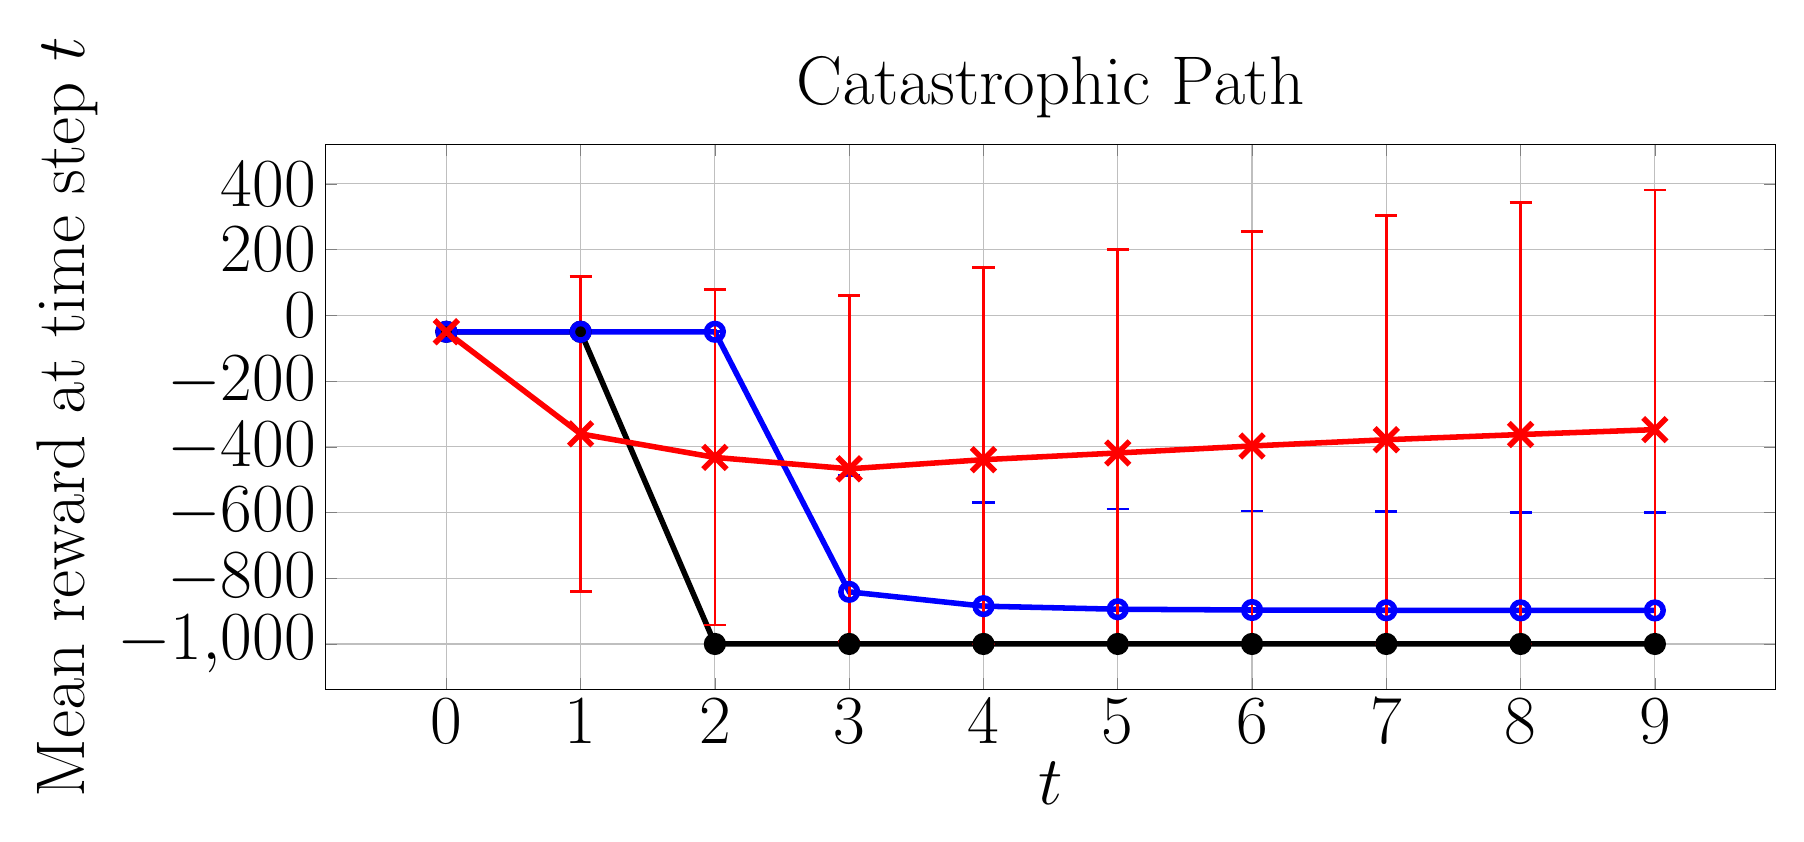
\begin{tikzpicture}
                \begin{axis}[
                    xlabel={$t$},
                    ylabel={Mean reward at time step $t$},
                    title={Catastrophic Path},
                    grid=both,
                    width=20cm, height=8.5cm,
                    every axis/.style={font=\Huge},
                    %
                ]
               \addplot[
                    color=black, %
                    mark=*, %
                    line width=2pt,
                    mark size=3pt,
                ]
                coordinates {
                    (0, -50.0)
                    (1, -50.0)
                    (2, -1000.0)
                    (3, -1000.0)
                    (4, -1000.0)
                    (5, -1000.0)
                    (6, -1000.0)
                    (7, -1000.0)
                    (8, -1000.0)
                    (9, -1000.0)
                };
                %
                %
                \addplot[
                    color=blue, %
                    mark=o, %
                    line width=2pt,
                    mark size=3pt,
                    error bars/.cd,
                    y dir=both, %
                    y explicit, %
                    error bar style={line width=1pt,solid},
                    error mark options={line width=1pt,mark size=4pt,rotate=90}
                ]
                coordinates {
                    (0, -50.0)  +- (0, 0.0)
                    (1, -50.0)  +- (0, 0.0) 
                    (2, -50.0)  +- (0, 0.0) 
                    (3, -841.440725)  += (0, 354.24605512) -= (0, 158.559275)
                    (4, -884.98225)  += (0, 315.37519669) -= (0, 115.01775)
                    (5, -894.330425) += (0, 304.88572805) -= (0, 105.669575)
                    (6, -896.696175) += (0, 301.19954514) -= (0, 103.303825)
                    (7, -897.4635) += (0, 299.61791279) -= (0, 102.5365)
                    (8, -897.77595) += (0, 298.80392585) -= (0, 102.22405)
                    (9, -897.942975) += (0, 298.32920557) -= (0, 102.057025)
                };
                %
                \addplot[
                    color=red, %
                    mark=x, %
                    line width=2pt,
                    mark size=6pt,
                    error bars/.cd,
                    y dir=both, %
                    y explicit, %
                    error bar style={line width=1pt,solid},
                    error mark options={line width=1pt,mark size=4pt,rotate=90}
                ]
            coordinates {
                    (0, -50.0)  +- (0, 0.0)
                    (1, -360.675265)  +- (0, 479.39812699) 
                    (2, -432.27629)  +- (0, 510.38620897) 
                    (3, -467.029545)  += (0, 526.36009628) -= (0, 526.36009628)
                    (4, -439.17429)  += (0, 583.96638919) -= (0, 560.82571)
                    (5, -418.82704) += (0, 618.43027478) -= (0, 581.17296)
                    (6, -397.464895) += (0, 652.67322574) -= (0, 602.535105)
                    (7, -378.49052) += (0, 682.85407033) -= (0, 621.50948)
                    (8, -362.654195) += (0, 707.01412023) -= (0, 637.345805)
                    (9, -347.737935) += (0, 729.29076479) -= (0, 652.262065)
                };
                %
                %
                %
                %
                %
                %
                %
                %
                %
                %
                %
                %
                %
                %
                %
                %
                %
                %
                %
                \end{axis}
            \end{tikzpicture}
         }
    }
    \caption{Average instant reward of CF paths induced by policies on Sepsis.}
    \label{fig: reward sepsis}
\end{figure*}

%
%
%
\subsection{Interval CFMDP Bounds}
%
%
Table \ref{tab:nonzero_probs} presents the mean counterfactual probability bound widths (excluding transitions where the upper bound is $0$) for each MDP, averaged over 20 observed paths. We compare the bounds under counterfactual stability (CS) and monotonicity (M) assumptions, CS alone, and no assumptions. This shows that the assumptions marginally reduce the bound widths, indicating the assumptions tighten the bounds without excluding too many causal models, as intended.
\renewcommand{\arraystretch}{1}

\begin{table}
\centering
\caption{Mean width of counterfactual probability bounds}
\resizebox{0.8\columnwidth}{!}{%
\begin{tabular}{|c|c|c|c|}
\hline
\multirow{2}{*}{\textbf{Environment}} & \multicolumn{3}{c|}{\textbf{Assumptions}} \\ \cline{2-4}
 & \textbf{CS + M} & \textbf{CS} & \textbf{None\tablefootnote{\jl{Equivalent to \citet{li2024probabilities}'s bounds (see Section \ref{sec: equivalence with Li}).}}} \\ \hline
\textbf{GridWorld} ($p=0.9$) & 0.0817 & 0.0977 & 0.100 \\ \hline
\textbf{GridWorld} ($p=0.4$) & 0.552  & 0.638  & 0.646 \\ \hline
\textbf{Sepsis} & 0.138 & 0.140 & 0.140 \\ \hline
\end{tabular}
}
\label{tab:nonzero_probs}
\end{table}


\subsection{Execution Times}
Table \ref{tab: times} compares the average time needed to generate the interval CFMDP vs.\ the Gumbel-max SCM CFMDP for 20 observations.
The GridWorld algorithms were run single-threaded, while the Sepsis experiments were run in parallel.
Generating the interval CFMDP is significantly faster as it uses exact analytical bounds, whereas the Gumbel-max CFMDP requires sampling from the Gumbel distribution to estimate counterfactual transition probabilities. \jl{Since constructing the counterfactual MDP models is the main bottleneck in both approaches, ours is more efficient overall and suitable for larger MDPs.}
\begin{table}
\centering
\caption{Mean execution time to generate CFMDPs}
\resizebox{0.99\columnwidth}{!}{%
\begin{tabular}{|c|c|c|}
\hline
\multirow{2}{*}{\textbf{Environment}} & \multicolumn{2}{c|}{\textbf{Mean Execution Time (s)}} \\ \cline{2-3} 
                                      & \textbf{Interval CFMDP} & \textbf{Gumbel-max CFMDP} \\ \hline
\textbf{GridWorld ($p=0.9$) }                  & 0.261                   & 56.1                      \\ \hline
\textbf{GridWorld ($p=0.4$)  }                 & 0.336                   & 54.5                      \\ \hline
\textbf{Sepsis}                                 & 688                     & 2940                      \\ \hline
\end{tabular}%
}
\label{tab: times}
\end{table}

\putsec{related}{Related Work}

\noindent \textbf{Efficient Radiance Field Rendering.}
%
The introduction of Neural Radiance Fields (NeRF)~\cite{mil:sri20} has
generated significant interest in efficient 3D scene representation and
rendering for radiance fields.
%
Over the past years, there has been a large amount of research aimed at
accelerating NeRFs through algorithmic or software
optimizations~\cite{mul:eva22,fri:yu22,che:fun23,sun:sun22}, and the
development of hardware
accelerators~\cite{lee:cho23,li:li23,son:wen23,mub:kan23,fen:liu24}.
%
The state-of-the-art method, 3D Gaussian splatting~\cite{ker:kop23}, has
further fueled interest in accelerating radiance field
rendering~\cite{rad:ste24,lee:lee24,nie:stu24,lee:rho24,ham:mel24} as it
employs rasterization primitives that can be rendered much faster than NeRFs.
%
However, previous research focused on software graphics rendering on
programmable cores or building dedicated hardware accelerators. In contrast,
\name{} investigates the potential of efficient radiance field rendering while
utilizing fixed-function units in graphics hardware.
%
To our knowledge, this is the first work that assesses the performance
implications of rendering Gaussian-based radiance fields on the hardware
graphics pipeline with software and hardware optimizations.

%%%%%%%%%%%%%%%%%%%%%%%%%%%%%%%%%%%%%%%%%%%%%%%%%%%%%%%%%%%%%%%%%%%%%%%%%%
\myparagraph{Enhancing Graphics Rendering Hardware.}
%
The performance advantage of executing graphics rendering on either
programmable shader cores or fixed-function units varies depending on the
rendering methods and hardware designs.
%
Previous studies have explored the performance implication of graphics hardware
design by developing simulation infrastructures for graphics
workloads~\cite{bar:gon06,gub:aam19,tin:sax23,arn:par13}.
%
Additionally, several studies have aimed to improve the performance of
special-purpose hardware such as ray tracing units in graphics
hardware~\cite{cho:now23,liu:cha21} and proposed hardware accelerators for
graphics applications~\cite{lu:hua17,ram:gri09}.
%
In contrast to these works, which primarily evaluate traditional graphics
workloads, our work focuses on improving the performance of volume rendering
workloads, such as Gaussian splatting, which require blending a huge number of
fragments per pixel.

%%%%%%%%%%%%%%%%%%%%%%%%%%%%%%%%%%%%%%%%%%%%%%%%%%%%%%%%%%%%%%%%%%%%%%%%%%
%
In the context of multi-sample anti-aliasing, prior work proposed reducing the
amount of redundant shading by merging fragments from adjacent triangles in a
mesh at the quad granularity~\cite{fat:bou10}.
%
While both our work and quad-fragment merging (QFM)~\cite{fat:bou10} aim to
reduce operations by merging quads, our proposed technique differs from QFM in
many aspects.
%
Our method aims to blend \emph{overlapping primitives} along the depth
direction and applies to quads from any primitive. In contrast, QFM merges quad
fragments from small (e.g., pixel-sized) triangles that \emph{share} an edge
(i.e., \emph{connected}, \emph{non-overlapping} triangles).
%
As such, QFM is not applicable to the scenes consisting of a number of
unconnected transparent triangles, such as those in 3D Gaussian splatting.
%
In addition, our method computes the \emph{exact} color for each pixel by
offloading blending operations from ROPs to shader units, whereas QFM
\emph{approximates} pixel colors by using the color from one triangle when
multiple triangles are merged into a single quad.


\section{Conclusion}
In this work, we propose a simple yet effective approach, called SMILE, for graph few-shot learning with fewer tasks. Specifically, we introduce a novel dual-level mixup strategy, including within-task and across-task mixup, for enriching the diversity of nodes within each task and the diversity of tasks. Also, we incorporate the degree-based prior information to learn expressive node embeddings. Theoretically, we prove that SMILE effectively enhances the model's generalization performance. Empirically, we conduct extensive experiments on multiple benchmarks and the results suggest that SMILE significantly outperforms other baselines, including both in-domain and cross-domain few-shot settings.

%% Acknowledgments
% \begin{acks}                            %% acks environment is optional
%   %% contents suppressed with 'anonymous'
%   %% Commands \grantsponsor{<sponsorID>}{<name>}{<url>} and
%   %% \grantnum[<url>]{<sponsorID>}{<number>} should be used to
%   %% acknowledge financial support and will be used by metadata
%   %% extraction tools.
%   This material is based upon work supported by the
%   \grantsponsor{GS100000001}{National Science
%     Foundation}{http://dx.doi.org/10.13039/100000001} under Grant
%   No.~\grantnum{GS100000001}{nnnnnnn} and Grant
%   No.~\grantnum{GS100000001}{mmmmmmm}.  Any opinions, findings, and
%   conclusions or recommendations expressed in this material are those
%   of the author and do not necessarily reflect the views of the
%   National Science Foundation.
% \end{acks}

%\newpage
\balance
% \bibliographystyle{plain}
\bibliography{refs}

\end{document}
